%% LyX 2.2.0 created this file.  For more info, see http://www.lyx.org/.
%% Do not edit unless you really know what you are doing.
\documentclass[english]{scrartcl}
\usepackage[T1]{fontenc}
\usepackage[latin9]{inputenc}
\usepackage{color}
\usepackage{babel}
\usepackage{array}
\usepackage{float}
\usepackage{multirow}
\usepackage{amsmath}
\usepackage{graphicx}
\usepackage[authoryear]{natbib}
\usepackage[unicode=true,pdfusetitle,
 bookmarks=true,bookmarksnumbered=false,bookmarksopen=false,
 breaklinks=false,pdfborder={0 0 1},backref=false,colorlinks=true]
 {hyperref}
\hypersetup{
 linkcolor=blue, urlcolor=blue, citecolor=blue}

\makeatletter

%%%%%%%%%%%%%%%%%%%%%%%%%%%%%% LyX specific LaTeX commands.
%% Because html converters don't know tabularnewline
\providecommand{\tabularnewline}{\\}
\floatstyle{ruled}
\newfloat{algorithm}{tbp}{loa}
\providecommand{\algorithmname}{Algorithm}
\floatname{algorithm}{\protect\algorithmname}

\makeatother

\begin{document}

\titlehead{\date{}Oct, 2017}

\subject{\href{http://parmes.github.io}{PARMES} - technical report - 2 -
revision - 1}

\title{A projected quasi-Newton method for dynamic multibody frictional
contact problems}
\maketitle
\begin{center}
{\Large{}Summary}
\par\end{center}{\Large \par}

We present a simple projected quasi-Newton approach for dealing with
frictional contact constraints in multibody dynamic simulations. A
regularized linear subproblem is solved inexactly at every Newton
step, rendering the method attractive in the context of parallel computations.
Our approach performs comparably with the commonly used Gauss-Seidel
scheme, while having a much lower communication cost in parallel.
We include examples of rigid and deformable problems, run on a distributed
memory cluster. An implementation of the presented method is available
at \href{https://parmes.github.io/solfec}{https://parmes.github.io/solfec}

\bigskip{}

\begin{center}
{\Large{}Contributors}
\par\end{center}{\Large \par}

\begin{center}
\begin{tabular}{c}
Tomasz Koziara, t.koziara@gmail.com\tabularnewline
\end{tabular}
\par\end{center}

\section{Introduction}

The motivation behind the presented work is in modeling the dynamics
of large collections of bodies interacting via contact and friction.
Our point of departure is Contact Dynamics, an implicit method originated
by Moreau \citep{Moreau01} and Jean \citep{Jean01}, facilitating
time integration with relatively large time steps. In order to solve
for contact reactions Contact Dynamics employs nonlinear Gauss-Seidel
relaxation. Although this approach is quite robust, its distributed
memory implementation requires much care \citep{Koziara2010}, and
can be inefficient when convergence is slow. In an earlier research
\citep{Koziara2008} we have looked into a nonsmooth Newton approach,
easier to parallelize, but representing potentially troublesome due
to oscillatory behavior. The current work proposes an alternative
formulation. We use the work of De Saxc\'e and Feng \citep{DeSaxce1998}
and modify the linearization by Fukushima et al. \citep{Fukushima2002}
in order to formulate the dynamic frictional contact problem as smooth
root finding. In order to find approximate solutions, we subsequently
develop a projected quasi-Newton method, which scales in parallel
and converges sufficiently well to replace the Gauss-Seidel approach
for the problem set of our interest. This approach may be useful in
a broader sense and hence it is documented in the current report.
We refer the reader to reviews \citep{Stewart2000,Brogliato2002}
for a perspective on finite-dimensional multibody contact/impact dynamics.
\href{http://epubs.siam.org/doi/10.1137/S0036144599360110}{The list of cross-references}
of review \citep{Stewart2000} may be helpful in tracking recent developments
in the field. For example a solution method by Mazhar et al. \citep{Mazhar2015}
has a similar character to the one presented here.

A brief account of discrete multibody dynamics is given in Section
\ref{sec:Discrete-dynamics}. Section \ref{sec:Frictional-contact}
formulates the frictional contact problem. Smoothing is discussed
in Section \ref{sec:Smoothing}. In Section \ref{sec:Constraints-satisfaction}
a convenient measure of accuracy is defined. Linearization is outlined
in Section \ref{sec:Linearization}. The projected quasi-Newton method
is detailed in Section \ref{sec:PQN}, followed by examples in Section
\ref{sec:Examples}. The paper is concluded in Section \ref{sec:Conclusions}.
In addition, Appendix \ref{sec:Derivative} includes derivation of
a smoothed derivative, while Appendix \ref{sec:Links} provides links
to source code and examples files.

\section{\label{sec:Discrete-dynamics}Discrete multibody dynamics}

At time $t$ a set of bodies has configuration $\mathbf{q}^{t}$ and
velocity $\mathbf{u}^{t}$. Consecutive values $\mathbf{q}^{t+h}$,
$\mathbf{u}^{t+h}$ for $h>0$ are obtained by numerical integration
of the momentum balance and the kinematic relation $\dot{\mathbf{q}}=\mathbf{u}$.
In order to focus attention, we briefly outline a scheme originally
presented in \citep{Moreau01}. A half-step configuration is obtained
as

\begin{equation}
\mathbf{q}^{t+h/2}=\mathbf{q}^{t}+\frac{h}{2}\mathbf{u}^{t}\mbox{.}\label{eq:q-half}
\end{equation}
The velocity update reads

\begin{equation}
\mathbf{u}^{t+h}=\mathbf{b}^{t+h}+\mathbf{A}^{-1}\mathbf{H}^{T}\mathbf{R}\label{eq:u}
\end{equation}
where

\begin{equation}
\mathbf{b}^{t+h}=\mathbf{u}^{t}+h\mathbf{A}^{-1}\mathbf{f}\label{eq:b}
\end{equation}
is a free velocity, not accounting for an influence of constraints.
When $\mathbf{A}=\mathbf{M}$, where $\mathbf{M}$ is an inertia matrix,
(\ref{eq:b}) corresponds to an explicit scheme detailed in \citep{Moreau01,Koziara2008PhD}.
For $\mathbf{A}=\mathbf{M}+\left(h^{2}/4\right)\mathbf{K}$, where
$\mathbf{K}=-\{\partial\mathbf{f}/\partial\mathbf{q}\}\left(\mathbf{q}^{t+h/2}\right)$
is a stiffness matrix, (\ref{eq:b}) corresponds to the linearly-implicit
scheme by Zhang and Skeel \citep{Zhang1997}. In both cases the out
of balance force $\mathbf{f}=\mathbf{f}\left(\mathbf{q}^{t+h/2},t+\frac{h}{2}\right)$.
For smooth problems both integrators have good conservation properties
and are of second order. Naturally, the linearly-implicit scheme allows
for larger time steps. While (\ref{eq:b}) represents a regular velocity
update for an unconstrained system, (\ref{eq:u}) accounts for the
constraints by adding a contribution of their reactions $\mathbf{R}$.
In (\ref{eq:u}) $\mathbf{A}=\mathbf{A}\left(\mathbf{q}^{t+h/2}\right)$
and $\mathbf{H}=\mathbf{H}\left(\mathbf{q}^{t+h/2}\right)$, while
$\mathbf{R}=\int_{t}^{t+h}d\mathbf{R}$ is considered to be an impulse.
$\mathbf{H}$ is a linear operator mapping the body space velocity
$\mathbf{u}$ into a constraint space velocity $\mathbf{U}$

\begin{equation}
\mathbf{U}=\mathbf{H}\mathbf{u}\mbox{.}\label{eq:H}
\end{equation}
For example, in case of finite elements, $\mathbf{H}$ is a global
to local coordinates transformation of the shape functions values
nonzero at constraint points. Once $\mathbf{R}$ is known, after obtaining
$\mathbf{u}^{t+h}$ the final configuration update reads 
\begin{equation}
\mathbf{q}^{t+h}=\mathbf{q}^{t+h/2}+\frac{h}{2}\mathbf{u}^{t+h}\mbox{.}\label{eq:q-end}
\end{equation}
In the remaining part of the paper we discuss how to calculate $\mathbf{R}$
in case of frictional contact constraints.

\section{\label{sec:Frictional-contact}Frictional contact formulation}

At $\mathbf{q}^{t+h/2}$ we identify a number of points where pairs
of bodies interact by contact. At those points, indexed by $\alpha$,
we introduce local coordinate systems. Each of those systems has an
axis pointing into the normal direction. This is the direction along
which bodies separate. The remaining two axes span a tangent plane.
This is the plane in which bodies shear. At each contact point, using
the local coordinate system, we consider a relative velocity $\mathbf{U}_{\alpha}$
and an impulse force $\mathbf{R}_{\alpha}$. Their relationship is
linear

\begin{equation}
\mathbf{U}_{\alpha}=\sum_{\beta}\mathbf{W}_{\alpha\beta}\mathbf{R}_{\beta}+\mathbf{B}_{\alpha}\label{eq:UWRB}
\end{equation}
where $\mathbf{W}_{\alpha\beta}$ are $3\times3$ block matrices and
$\mathbf{B}_{\alpha}$ are $3$-vectors contributing to

\begin{equation}
\mathbf{W}=\mathbf{H}\mathbf{A}^{-1}\mathbf{H}^{T}\label{eq:W}
\end{equation}

\begin{equation}
\mathbf{B}=\mathbf{H}\mathbf{b}^{t+h}
\end{equation}
in a suitable manner. Because for $\mathbf{R}=\mathbf{0}$ there holds
$\mathbf{U}=\mathbf{B}$, $\mathbf{B}$ is the free relative velocity
at the constraints.

At contact points we consider a minimalistic interface law, reflecting
the core difficulties related to the lack of smoothness and the non-associated
character of friction. In terms of normal behaviour we employ the
velocity Signorini condition, $U_{\alpha N}\ge0,\,\,\,R_{\alpha N}\ge0,\,\,\,U_{\alpha N}R_{\alpha N}=0$.
In terms of shearing behavior we utilize the Coulomb law, $\mathbf{R}_{\alpha}\in\mbox{interior}\left(K_{\alpha}\right)\Rightarrow\mathbf{U}_{\alpha T}=0$
and $\mathbf{R}_{\alpha}\in\mbox{boundary}\left(K_{\alpha}\right)\Rightarrow\mathbf{U}_{\alpha T}=-\gamma\mathbf{R}_{\alpha T}$,
where $\gamma>0$. The friction cone $K_{\alpha}$ is defined as

\begin{equation}
K_{\alpha}=\left\{ \mathbf{R}_{\alpha}:\left\Vert \mathbf{R}_{\alpha T}\right\Vert \le\mu_{\alpha}R_{\alpha N},R_{\alpha N}\ge0\right\} 
\end{equation}
where $\mu_{\alpha}$ is the coefficient of friction. It has been
shown by De Saxc\'e and Feng \citep{DeSaxce1998}, that the Signorini-Coulomb
law can be expressed in a compact form

\begin{equation}
-\left[\begin{array}{c}
\mathbf{U}_{\alpha T}\\
U_{\alpha N}+\mu_{\alpha}\left\Vert \mathbf{U}_{\alpha T}\right\Vert 
\end{array}\right]\in N_{K_{\alpha}}\left(\mathbf{R}_{\alpha}\right)\label{eq:DSF}
\end{equation}
where $N_{K_{\alpha}}$ stands for the normal cone of the set $K_{\alpha}$.
For a convex set $A$ the normal cone $N_{A}\left(\mathbf{R}\right)$
at point $\mathbf{R}\in A$ is defined as the set of all vectors $\mathbf{V}$
such that $\left\langle \mathbf{V},\mathbf{S}-\mathbf{R}\right\rangle \le0$
for all $\mathbf{S}\in A$. Let us now define

\begin{equation}
\mathbf{F}\left(\mathbf{R}\right)=\left[\begin{array}{c}
...\\
\mathbf{U}_{\alpha T}\left(\mathbf{R}\right)\\
U_{\alpha N}\left(\mathbf{R}\right)+\mu_{\alpha}\left\Vert \mathbf{U}_{\alpha T}\left(\mathbf{R}\right)\right\Vert \\
...
\end{array}\right]\label{eq:F}
\end{equation}
and

\begin{equation}
K=\prod_{\alpha}K_{\alpha}
\end{equation}
where the dependence $\mathbf{U}_{\alpha}\left(\mathbf{R}\right)$
is defined in (\ref{eq:UWRB}), and $\mathbf{R}$ is a collection
of $\mathbf{R}_{\alpha}$ for $\alpha\in\left\{ 1,...,\nu\right\} $.
Formula (\ref{eq:DSF}) states, that the frictional contact constraints
are satisfied if $-\mathbf{F}\left(\mathbf{R}\right)$ belongs to
the normal cone of $K$ at $\mathbf{R}$. Hence

\begin{equation}
-\mathbf{F}\left(\mathbf{R}\right)=\mathbf{R}-\mathbf{F}\left(\mathbf{R}\right)-\mbox{proj}_{K}\left(\mathbf{R}-\mathbf{F}\left(\mathbf{R}\right)\right)
\end{equation}
which can be reduced to the standard projection formula $\mathbf{R}=\mbox{proj}_{K}\left(\mathbf{R}-\mathbf{F}\left(\mathbf{R}\right)\right)$.
Let us not do it though, but rather define a vector field

\begin{equation}
\mathbf{m}\left(\mathbf{S}\right)=\mathbf{S}-\mbox{proj}_{K}\left(\mathbf{S}\right)\mbox{.}
\end{equation}
We can rewrite (\ref{eq:DSF}) as

\begin{equation}
\mathbf{C}\left(\mathbf{R}\right)=\mathbf{F}\left(\mathbf{R}\right)+\mathbf{m}\left(\mathbf{R}-\mathbf{F}\left(\mathbf{R}\right)\right)=\mathbf{0}\mbox{ and }\mathbf{R}\in K\mbox{,}\label{eq:C1}
\end{equation}
a root finding problem defined within the friction cone.

\section{\label{sec:Smoothing}Smoothing}

Projection is a nonsmooth operator and so is $\mathbf{m}\left(\mathbf{S}\right)$.
Similarly, $\mathbf{F}\left(\mathbf{R}\right)$ is not smooth due
to $\left\Vert \mathbf{U}_{\alpha T}\left(\mathbf{R}\right)\right\Vert $.
Since our aim to to develop a Newton-like approach for equation (\ref{eq:C1}),
some suitable notion of derivative needs to be put in place. Plethora
of nonsmooth analytical tools have been developed in recent decades,
many of which are summarized in the monograph \citep{RW98}. This
avenue has been investigated in our previous work \citep{Koziara2008}.
In this paper we are interested in exploring the classical smooth
toolbox and hence we adopt the work of Fukushima at al. \citep{Fukushima2002}
in the context of frictional contact. Since we shall need a gradient
of $\mathbf{C}\left(\mathbf{R}\right)$, our first step is to produce
its smooth approximation $\mathbf{C}_{\omega}\left(\mathbf{R}\right)$,
such that $\nabla\mathbf{C}_{\omega}\left(\mathbf{R}\right)$ is well
defined for all $\omega>0$.

\subsection{Smoothed $\mathbf{m}\left(\mathbf{S}\right)$}

A polar cone $K_{\alpha}^{\circ}$ of the friction cone $K_{\alpha}$
is defined as follows

\begin{equation}
K_{\alpha}^{\circ}=\left\{ \mathbf{V}:\left\langle \mathbf{V},\mathbf{S}\right\rangle \le0\mbox{ for all }\mathbf{S}\in K_{\alpha}\right\} =N_{K_{\alpha}}\left(\mathbf{0}\right)\mbox{.}
\end{equation}
For any $\mathbf{S}_{\alpha}$ we have (Moreau)

\begin{equation}
\mathbf{S}_{\alpha}=\mbox{proj}_{K_{\alpha}}\left(\mathbf{S}_{\alpha}\right)+\mbox{proj}_{K_{\alpha}^{\circ}}\left(\mathbf{S}_{\alpha}\right)
\end{equation}
and hence

\begin{equation}
\mathbf{m}_{\alpha}\left(\mathbf{S}_{\alpha}\right)=\mbox{proj}_{K_{\alpha}^{\circ}}\left(\mathbf{S}_{\alpha}\right)\mbox{.}
\end{equation}
We use the analysis from \citep{Fukushima2002} in order to derive
a smoothed $\mathbf{m}\left(\mathbf{S}\right)$. In \citep{Fukushima2002}
only the self-dual case $\mu_{\alpha}=1$ was considered. The formulas
obtained here represent a slight generalization. In order to avoid
clutter, we temporarily omit the $\alpha$-indexing of contact point
entities. For any $\mathbf{z}\in R^{3}$ we define the following spectral
factorization with respect to the pair of cones $-K$ and $K^{\circ}$

\begin{equation}
\mathbf{z}=\lambda_{1}\mathbf{u}_{1}+\lambda_{2}\mathbf{u}_{2}
\end{equation}
where $\lambda_{1}$, $\lambda_{2}$ are spectral values

\begin{equation}
\lambda_{1}=\frac{-z_{N}-\mu\left\Vert \mathbf{z}_{T}\right\Vert }{1+\mu^{2}},\,\,\,\lambda_{2}=\frac{\left\Vert \mathbf{z}_{T}\right\Vert -\mu z_{N}}{1+\mu^{2}}\label{eq:l12}
\end{equation}
and $\mathbf{u}_{1}$, $\mathbf{u}_{2}$ are spectral vectors

\begin{equation}
\mathbf{u}_{1}=\left\{ \begin{array}{ccc}
\left[\begin{array}{c}
-\mu\frac{\mathbf{z}_{T}}{\left\Vert \mathbf{z}_{T}\right\Vert }\\
-1
\end{array}\right] & \mbox{if} & \mathbf{z}_{T}\ne\mathbf{0}\\
\left[\begin{array}{c}
-\mu\mathbf{w}\\
-1
\end{array}\right] & \mbox{if} & \mathbf{z}_{T}=\mathbf{0}
\end{array}\right.\label{eq:u1}
\end{equation}

\begin{equation}
\mathbf{u}_{2}=\left\{ \begin{array}{ccc}
\left[\begin{array}{c}
\frac{\mathbf{z}_{T}}{\left\Vert \mathbf{z}_{T}\right\Vert }\\
-\mu
\end{array}\right] & \mbox{if} & \mathbf{z}_{T}\ne\mathbf{0}\\
\left[\begin{array}{c}
\mathbf{w}\\
-\mu
\end{array}\right] & \mbox{if} & \mathbf{z}_{T}=\mathbf{0}
\end{array}\right.\label{eq:u2}
\end{equation}
where $\mathbf{w}\in R^{2}$ and $\left\Vert \mathbf{w}\right\Vert =1$.
For any $\mathbf{z}\in R^{3}$ we can write

\begin{equation}
\mbox{proj}_{K^{\circ}}\left(\mathbf{z}\right)=\max\left(0,\lambda_{1}\right)\mathbf{u}_{1}+\max\left(0,\lambda_{2}\right)\mathbf{u}_{2}\label{eq:proj_K_po}
\end{equation}
where $\lambda_{1},\lambda_{2}$ and $\mathbf{u}_{1},\mathbf{u}_{2}$
are defined in (\ref{eq:l12}), (\ref{eq:u1}) and (\ref{eq:u2}).
For any $\mathbf{z}\in R^{3}$ with $\mathbf{z}_{T}\ne\mathbf{0}$
we take a slice of $R^{3}$ and span a Cartesian $x$-$y$ frame along
$\mathbf{z}_{T}$ and $\left[0,0,1\right]^{T}$ respectively. Then
$x_{\mathbf{z}}>0$, $\mathbf{u}_{1}$ corresponds to a $x$-negative
face of $K^{\circ}$ and $\mathbf{u}_{2}$ corresponds to a $x$-positive
face of $-K$. Clearly, $\mathbf{u}_{1}\perp\mathbf{u}_{2}$ and $\lambda_{1}$
and $\lambda_{2}$ are the normalized projections of $\mathbf{z}$
onto these two directions. Formula (\ref{eq:proj_K_po}) follows from
the geometry of $-K$ and $K^{\circ}$.

The projection operator as defined in (\ref{eq:proj_K_po}) is nonsmooth.
Motivated by \citep{Fukushima2002,Hayashi2005} we employ the following
smoothing

\begin{equation}
\mbox{proj}_{K^{\circ}}^{\omega}\left(\mathbf{z}\right)=\omega g\left(\lambda_{1}/\omega\right)\mathbf{u}_{1}+\mu\omega g\left(\lambda_{2}/\left(\mu\omega\right)\right)\mathbf{u}_{2}\label{eq:proj_K_ps}
\end{equation}
where

\begin{equation}
g\left(\lambda\right)=\frac{1}{2}\left(\sqrt{\lambda^{2}+4}+\lambda\right)\mbox{.}\label{eq:g}
\end{equation}
The smoothing function $\omega g\left(\lambda/\omega\right)$ is differentiable
for all $\omega>0$ and it converges to $\max\left(0,\lambda\right)$
when $\omega\downarrow0$. There also hold

\begin{equation}
\lim_{\lambda\rightarrow-\infty}g\left(\lambda\right)=0,\,\,\,\lim_{\lambda\rightarrow\infty}(g\left(\lambda\right)-\lambda)=0,\,\,\,0<\dot{g}\left(\lambda\right)<1
\end{equation}
mimicking the behavior of $\max\left(0,\lambda\right)$. The gradient
of the smoothed projection onto the polar cone reads

\begin{equation}
\nabla\mbox{proj}_{K^{\circ}}^{\omega}\left(\mathbf{z}\right)=\left\{ \begin{array}{ccc}
\dot{g}\left(\lambda_{1}/\omega\right)\mathbf{I} & \mbox{if} & \mathbf{z}_{T}=\mathbf{0}\\
\left[\begin{array}{cc}
a\mathbf{I}+\left(b-a\right)\mathbf{z}_{T}\mathbf{z}_{T}^{T}/\left\Vert \mathbf{z}_{T}\right\Vert ^{2} & c\mathbf{z}_{T}/\left\Vert \mathbf{z}_{T}\right\Vert \\
c\mathbf{z}_{T}^{T}/\left\Vert \mathbf{z}_{T}\right\Vert  & d
\end{array}\right] & \mbox{if} & \mathbf{z}_{T}\ne\mathbf{0}
\end{array}\right.\label{eq:grad_proj}
\end{equation}
where

\begin{equation}
a=\frac{g\left(\lambda_{2}/\left(\mu\omega\right)\right)-g\left(\lambda_{1}/\omega\right)}{\lambda_{2}/\left(\mu\omega\right)-\lambda_{1}/\omega},b=\frac{\mu^{2}\dot{g}\left(\lambda_{1}/\omega\right)+\dot{g}\left(\lambda_{2}/\left(\mu\omega\right)\right)}{1+\mu^{2}}\label{eq:ab1}
\end{equation}

\begin{equation}
c=\frac{\mu\left(\dot{g}\left(\lambda_{1}/\omega\right)-\dot{g}\left(\lambda_{2}/\left(\mu\omega\right)\right)\right)}{1+\mu^{2}},d=\frac{\dot{g}\left(\lambda_{1}/\omega\right)+\mu^{2}\dot{g}\left(\lambda_{2}/\left(\mu\omega\right)\right)}{1+\mu^{2}}\mbox{.}\label{eq:cd1}
\end{equation}
A detailed derivation of the above formula can be found in Appendix
2, where after \citep{Fukushima2002,Hayashi2005} we also show that
$\nabla\mbox{proj}_{K^{\circ}}^{\omega}$ is positive definite for
$\omega>0$. Finally, the smoothed $\mathbf{m}\left(\mathbf{S}\right)$
reads

\begin{equation}
\mathbf{m}_{\omega}\left(\mathbf{S}\right)=\mbox{proj}{}_{K^{\circ}}^{\omega}\left(\mathbf{S}\right)\mbox{.}
\end{equation}


\subsubsection{Zero friction}

It is instructive to investigate the behavior of $\mathbf{m}_{\omega}\left(\mathbf{S}\right)$
and its gradient in the limit case of $\mu=0$. For $g_{1}=\omega g\left(\lambda_{1}/\omega\right)$
and $g_{2}=\mu\omega g\left(\lambda_{2}/\left(\mu\omega\right)\right)$
we have

\begin{equation}
g_{1}=\frac{1}{2}\left(\lambda_{1}+\sqrt{\lambda_{1}^{2}+4\omega^{2}}\right),g_{2}=\frac{1}{2}\left(\lambda_{2}+\sqrt{\lambda_{2}^{2}+4\mu^{2}\omega^{2}}\right)
\end{equation}
and hence

\begin{equation}
\mathbf{m}_{\omega}\left(\mathbf{S}\right)=g_{1}\mathbf{u}_{1}+\max\left(0,\lambda_{2}\right)\mathbf{u}_{2}\mbox{.}
\end{equation}
The tangential direction $\mathbf{u}_{2}$ is not active in the frictionless
case and it is not smoothed. For $\mu=0$ the tangential component
of $\mathbf{C}\left(\mathbf{R}\right)$ reads

\begin{equation}
\mathbf{C}_{T}\left(\mathbf{R}\right)=\mathbf{F}_{T}\left(\mathbf{R}\right)+\mathbf{m}_{T}\left(\mathbf{R}-\mathbf{F}\left(\mathbf{R}\right)\right)=\mathbf{R}_{T}
\end{equation}
and hence $\mathbf{C}_{T}\left(\mathbf{R}\right)=\mathbf{0}$ implies
$\mathbf{R}_{T}=\mathbf{0}$. This is also reflected in $\nabla_{\omega}\mathbf{m}\left(\mathbf{S}\right)$
and consequently in $d\mathbf{C}_{\omega}\left(\mathbf{U},\mathbf{R}\right)=\nabla_{\omega}\mathbf{m}\left(\mathbf{R}-\mathbf{U}\right)d\mathbf{R}$,
since $\nabla\mathbf{F}\left(\mathbf{U}\right)=\mathbf{I}$ for $\mu=0$.
Let us produce practical versions of (\ref{eq:ab1}) and (\ref{eq:cd1})
first. We have

\begin{equation}
\dot{g}_{1}=\frac{1}{2}\left(1+\lambda_{1}/\sqrt{\lambda_{1}^{2}+4\omega^{2}}\right),\dot{g}_{2}=\frac{1}{2}\left(1+\lambda_{2}/\sqrt{\lambda_{2}^{2}+4\mu^{2}\omega^{2}}\right)
\end{equation}
and

\begin{equation}
a=\frac{1}{2}\left(1+\left(\lambda_{2}+\mu\lambda_{1}\right)/\left(\sqrt{\lambda_{2}^{2}+4\mu^{2}\omega^{2}}+\mu\sqrt{\lambda_{1}^{2}+4\omega^{2}}\right)\right)
\end{equation}

\begin{equation}
b=\left(\mu^{2}\dot{g}_{1}+\dot{g}_{2}\right)/\left(1+\mu^{2}\right)
\end{equation}

\begin{equation}
c=\mu\left(\dot{g}_{1}-\dot{g}_{2}\right)/\left(1+\mu^{2}\right)
\end{equation}

\begin{equation}
d=\left(\dot{g}_{1}+\mu^{2}\dot{g}_{2}\right)/\left(1+\mu^{2}\right)\mbox{.}
\end{equation}
In case of $\mathbf{z}_{T}=\mathbf{R}_{T}-\mathbf{F}\left(\mathbf{R}\right)_{T}=\mathbf{0}$
the gradient is well defined in (\ref{eq:grad_proj}). Otherwise it
is quite easy to see that $a=b=1$, $c=0$, $d=\dot{g}\left(\lambda_{1}/\omega\right)$
and again $\nabla\mathbf{m}_{\omega}\left(\mathbf{S}\right)$ is well
defined.

\subsection{Smoothed $\mathbf{F}\left(\mathbf{R}\right)$}

The smoothed $\mathbf{F}\left(\mathbf{R}\right)$ reads

\begin{equation}
\mathbf{F}_{\omega}\left(\mathbf{U}\right)=\left[\begin{array}{c}
...\\
\mathbf{U}_{\alpha T}\\
U_{\alpha N}+\mu_{\alpha}\left(\sqrt{\left\langle \mathbf{U}_{\alpha T},\mathbf{U}_{\alpha T}\right\rangle +\omega^{2}}-\omega\right)\\
...
\end{array}\right]
\end{equation}
so that $\nabla\mathbf{F}_{\omega}$ is well defined for any $\omega>0$
and the smoothed norm $\left\Vert \mathbf{U}_{T}\right\Vert _{\omega}=\sqrt{\left\langle \mathbf{U}_{T},\mathbf{U}_{T}\right\rangle +\omega^{2}}-\omega=0$
for $\mathbf{U}_{T}=\mathbf{0}$. 

\section{\label{sec:Constraints-satisfaction}Constraints satisfaction measure}

For $\mathbf{R}\in K$ the vector function $\mathbf{C}\left(\mathbf{R}\right)=\mathbf{F}\left(\mathbf{R}\right)+\mathbf{m}\left(\mathbf{R}-\mathbf{F}\left(\mathbf{R}\right)\right)$
represents the relative velocity at contact points, which is not compatible
with the Signorini-Coulomb frictional contact law. It is therefore
possible to define a measure of constraints satisfaction, that has
some physical interpretation. Because\textbf{ }$\mathbf{C}$ is expressed
in terms of velocity, the following quantity

\begin{equation}
g\left(\mathbf{R}\right)=\sum_{\alpha=1}^{\nu}\left\langle \mathbf{W}_{\alpha\alpha}^{-1}\mathbf{C}_{\alpha}\left(\mathbf{R}\right),\mathbf{C}_{\alpha}\left(\mathbf{R}\right)\right\rangle /\sum_{\alpha=1}^{\nu}\left\langle \mathbf{W}_{\alpha\alpha}^{-1}\mathbf{B}_{\alpha},\mathbf{B}_{\alpha}\right\rangle \label{eq:accuracy}
\end{equation}
approximately measures the amount of spurious energy, due to an inexact
satisfaction of constraints. The denominator corresponds to the kinetic
energy of the relative free motion. $\mathbf{W}_{\alpha\alpha}$ are
the diagonal, $3\times3$, positive definite blocks of $\mathbf{W}$.
The above formula has already been used in \citep{Koziara2010}. It
can be used to compare the accuracy of solutions obtained by means
of different numerical approaches. The merit function $g\left(\mathbf{R}\right)$
is used in Section \ref{sec:PQN} as a termination criterion for the
projected quasi-Newton scheme. This is one among many possible choices
(not necessarily the best). Selecting a good convergence criterion
for ill-conditioned problems that are often generated by multibody
frictional contact formulations remains an open issue. Other termination
criteria has been discussed for example in \citep{Renouf2005,Radjai2009}.

\section{\label{sec:Linearization}Linearization}

When linearizing the problem it is useful to think of $\mathbf{U}$
and $\mathbf{R}$ as independent and write

\begin{equation}
\mathbf{C}_{\omega}\left(\mathbf{U},\mathbf{R}\right)=\mathbf{F}_{\omega}\left(\mathbf{U}\right)+\mathbf{m}_{\omega}\left(\mathbf{R}-\mathbf{F}_{\omega}\left(\mathbf{U}\right)\right),\mathbf{U}=\mathbf{W}\mathbf{R}+\mathbf{B}\mbox{,}
\end{equation}
We then have

\begin{equation}
d\mathbf{C}_{\omega}=\mathbf{X}d\mathbf{U}+\mathbf{Y}d\mathbf{R}
\end{equation}
where $\mathbf{X}$ and $\mathbf{Y}$ are $3\times3$-block diagonal
matrices

\begin{equation}
\mathbf{X}=\left[\mathbf{I}-\partial\mathbf{m}_{\omega}/\partial\mathbf{S}\right]\partial\mathbf{F}_{\omega}/\partial\mathbf{U}
\end{equation}

\begin{equation}
\mathbf{Y}=\partial\mathbf{m}_{\omega}/\partial\mathbf{S}
\end{equation}
and $\mathbf{I}$ is identity. The linearization reads

\begin{equation}
\mathbf{U}=\mathbf{W}\mathbf{R}+\mathbf{B}
\end{equation}

\begin{equation}
\mathbf{C}_{\omega}\left(\mathbf{U},\mathbf{R}\right)+\mathbf{X}d\mathbf{U}+\mathbf{Y}d\mathbf{R}=0
\end{equation}

\begin{equation}
d\mathbf{U}=\mathbf{W}d\mathbf{R}\mbox{.}
\end{equation}
By eliminating $\mathbf{U}$ and $d\mathbf{U}$ we come back to $\mathbf{C}_{\omega}\left(\mathbf{R}\right)=\mathbf{C}_{\omega}\left(\mathbf{W}\mathbf{R}+\mathbf{B},\mathbf{R}\right)$
and see that in the linearization of $\mathbf{C}_{\omega}\left(\mathbf{R}\right)=\mathbf{0}$,

\begin{equation}
\mathbf{C}_{\omega}\left(\mathbf{R}\right)+\nabla\mathbf{C}_{\omega}\left(\mathbf{R}\right)d\mathbf{R}=0\mbox{,}
\end{equation}
the gradient reads

\begin{equation}
\nabla\mathbf{C}_{\omega}\left(\mathbf{R}\right)=\mathbf{X}\mathbf{W}+\mathbf{Y}\mbox{.}\label{eq:Grad_C}
\end{equation}
It is noteworthy, that when using an iterative solver $\nabla\mathbf{C}_{\omega}$
does not need to be fully assembled. On the other hand it is clear
that $\nabla\mathbf{C}_{\omega}$ and $\mathbf{W}$ have the same
pattern of sparsity.

\section{\label{sec:PQN}Projected quasi-Newton method}

Our idea is to employ the following projected quasi-Newton step

\begin{equation}
\mathbf{R}^{k+1}=\mbox{proj}_{K}\left[\mathbf{R}^{k}-\mathbf{A}^{-1}\mathbf{C}_{\omega}\left(\mathbf{R}^{k}\right)\right]\label{eq:newton}
\end{equation}
where

\begin{equation}
\mathbf{A}\simeq\nabla\mathbf{C}_{\omega}\left(\mathbf{R}^{k}\right)
\end{equation}
is an approximation of $\nabla\mathbf{C}_{\omega}$. Since in many
practical situations $\nabla\mathbf{C}_{\omega}$ is singular (locally
or globally there may be more constraints than kinematic freedom),
we cannot hope for directly employing $\nabla\mathbf{C}_{\omega}$.
The projection is required by (\ref{eq:C1}), so that the iterates
remain within the friction cone. For the sake of simplicity the only
strategy that we wish to use to achieve a global convergence is the
combination of the projection and a suitable choice of $\mathbf{A}$.

Perhaps the simplest regularization of $\nabla\mathbf{C}_{\omega}$
is a diagonal perturbation

\begin{equation}
\mathbf{A}=\nabla\mathbf{C}_{\omega}+\delta\mathbf{I}
\end{equation}
where $\delta>0$. After combining it with an approximate, iterative
inversion of $\mathbf{A}$, we end up with the following projected
quasi-Newton step

\begin{equation}
\mathbf{R}^{k+1}=\mbox{proj}_{K}\left[\mathbf{R}^{k}-\left(\nabla\mathbf{C}_{\omega}^{k}+\delta\mathbf{I}\right)_{\mbox{GMRES}\left(\epsilon\left\Vert \mathbf{C}_{\omega}^{k}\right\Vert ,m\right)}^{-1}\mathbf{C}_{\omega}^{k}\right]
\end{equation}
where by $\mathbf{C}_{\omega}^{k}$ and $\nabla\mathbf{C}_{\omega}^{k}$
we mean the values taken at $\mathbf{R}^{k}$. In more detail the
above formula is presented as Algorithm \ref{alg:PQN}. In step (a)
we update the velocity $\mathbf{U}^{k}$. This is needed in order
to compute $\mathbf{C}_{\omega}^{k}$ and $\nabla\mathbf{C}_{\omega}^{k}$
in step (b). The GMRES solver runs with the absolute accuracy $\epsilon\left\Vert \mathbf{C}_{\omega}^{k}\right\Vert $
and the iterations bound $m$ in step (c). Importantly, GMRES is preconditioned
with inverted diagonal $3\times3$ blocks of $\mathbf{A}$. Finally
the projection step follows in (d). We note, that the parallel communication
is required in steps (a) and (c) for the matrix-vector products, and
in the last line of the algorithm to add up values of $g\left(\mathbf{R}^{k}\right)$
from different processors.

No numerical scheme is 100\% robust and in the last line of Algorithm
\ref{alg:PQN} we fall back on the Gauss-Seidel scheme \citep{Koziara2010}
when Newton iterations fail. Quality of contact solution often depends
on the quality of contact points and it is not uncommon that ill-conditioned
or contradictory contact points are produced in multibody simulations.
In such cases the Gauss-Seidel scheme generates a good approximate
solution, while the Newton solver may have terminated rather far off.

\begin{algorithm}
\begin{description}
\item [{PQN($\mathbf{R},\gamma,n,\omega,\delta,m,\epsilon$):}]~
\end{description}
\begin{enumerate}
\item $\triangle\mathbf{R}^{0}=\mathbf{0}$, $k=0$.
\item Do

\begin{enumerate}
\item $\mathbf{U}^{k}=\mathbf{W}\mathbf{R}^{k}+\mathbf{B}$.
\item Compute $\mathbf{C}_{\omega}^{k}$ and $\mathbf{A}^{k}=\nabla\mathbf{C}_{\omega}^{k}+\delta\mathbf{I}$.
\item $\triangle\mathbf{R}^{k}=\left(\mathbf{A}^{k}\right)_{\mbox{GMRES}\left(\epsilon\left\Vert \mathbf{C}_{\omega}^{k}\right\Vert ,m\right)}^{-1}\mathbf{C}_{\omega}^{k}$.
\item $\mathbf{R}^{k+1}=\mbox{proj}_{K}\left[\mathbf{R}^{k}-\triangle\mathbf{R}^{k}\right]$.
\item $k=k+1$.
\end{enumerate}
while $g\left(\mathbf{R}^{k}\right)\ge\gamma$ and $k<n$.
\item If $k=n$ then use the Gauss-Seidel solver from \citep{Koziara2010}.
\end{enumerate}
\caption{\label{alg:PQN}The projected quasi-Newton method.}
\end{algorithm}

We do not attempt to analyze the convergence of the presented scheme.
From our experience, proofs of global convergence for nonmonotone
problems ($\mu>0$) rarely bear relevance to numerical practice. On
the other hand, for well behaved problems ($\mu=0$) almost all methods
work, be it smooth or nonsmooth. For completeness we mention that
the globalization strategy adopted here has been analyzed under the
name of pseudo-transient continuation \citep{Kelley1998}.

\section{\label{sec:Examples}Examples}

Two examples are presented: a rotating drum of rigid or pseudo-rigid
ellipsoids and a sine sweep excitation of stacked finite element cubes.
In the examples, when not mentioned otherwise, default parameters
from Table \ref{tab:defs} are employed in Algorithm \ref{alg:PQN}. 

\begin{table}
\begin{centering}
\begin{tabular}{|c|c|c|c|c|c|c|c|}
\hline 
$\gamma$ & $n$ & $\omega$ & $\delta$ & $m$ & $\epsilon$ & GMRES restart & MV products\tabularnewline
\hline 
1E-8 & 1000 & $\mbox{1E-3}\cdot\gamma$ & 0 & 10 & 0.25 & 20 & 100000\tabularnewline
\hline 
\end{tabular}
\par\end{centering}
\caption{\label{tab:defs}Default parameter values for Algorithm \ref{alg:PQN}.
GMRES restart corresponds to the fixed size of the Krylov subspace
used by the GMRES solver. MV products is the upper bound on the total
number of matrix-vector products performed by GMRES.}
\end{table}


\subsection{Rotating drum of rigid and pseudo-rigid ellipsoids}

This example illustrates a motion of particles inside of a rotating
drum. The drum geometry is depicted in Figure \ref{fig:drum0} (a):
the drum is made out of a hollow pipe with inner radius of 1.0m and
thickness 0.05m, spanned between points $\left(0,0,0\right)$ and
$\left(0,0.5,0\right)$, and subdivided into 32 flat pieces. There
are two rectilinear blocks, centered at points $\left(-0.9,0.25,0\right)$
and $\left(0.9,0.25,0\right)$, of size $0.2\times0.5\times0.2$ along
the x, y, z directions. The drum is modeled as an obstacle - meaning
that its mass is not contributing to the simulated physics of the
problem. Two side walls are used to prevent falling out of particles
(disk shaped obstacles, not shown in the figure). There are two stages
of the simulation: dropping down the particles and rotating the drum.
Figure \ref{fig:drum0} (b) illustrates the particle dropping stage:
the user specifies the number of particles $N$ and the radii of the
particles is determined as follows:

\[
r_{0}=(0.1/N)^{1/3},\,r_{x}=0.9r_{0},r_{y}=0.5r_{0},r_{z}=r_{0},\,r_{1}=\frac{r_{x}+r_{y}+r_{z}}{3}
\]
where $r_{x}$, $r_{y}$, $r_{z}$ are the radii of ellipsoidal particles
and $r_{1}$ is a radii of spherical particles (when used below).
Particles are first dropped down until all $N$ of them are inserted
into the simulation. The drum begins to rotate next. The total simulation
time is $10$ seconds and the time step is $0.001$ second (unless
specified otherwise). The particle material parameters are $E=1\text{E6Pa}$,
$\mu=0.25$, $\rho=100\text{kg}/\text{m}^{3}$ for the Young modulus,
Poisson ratio and mass density, respectively. Gravity is $\left(0,0,-10\right)$.
The angular velocity of rotation is $\left(0,1,0\right)\text{rad/s}$
(unless specified otherwise). The Signoroni-Coulomb material model
\citep{Jean01} is used and the coefficient of friction is $0.3$.
Two kinematic models are used in this example: rigid and pseudo-rigid
\citep{CM88}. In the latter case the rotation matrix of the rigid
model is replaced by a $3\times3$ linear transformation (per-body
deformation gradient) and hence the ellipsoids deform linearly (develop
constant strain/stress). When labeling results reported below by \emph{ell.
rigid} we mean simulations involving rigid ellipsoids, while by \emph{ell.
defo} we mean simulations involving pseudo-rigid ellipsoids; \emph{sph.
rigid} and \emph{sph. defo} are used analogously when spherical particles
are used instead. The elliptical pseudo-rigid particles (\emph{ell.
defo}) actually deform: their geometry is updated based on the current
deformation gradient. The spherical pseudo-rigid particles (\emph{shp.
defo}) are updated in a simplified manner: their initial spherical
shape is retained.

\begin{figure}[h]
\begin{centering}
(a)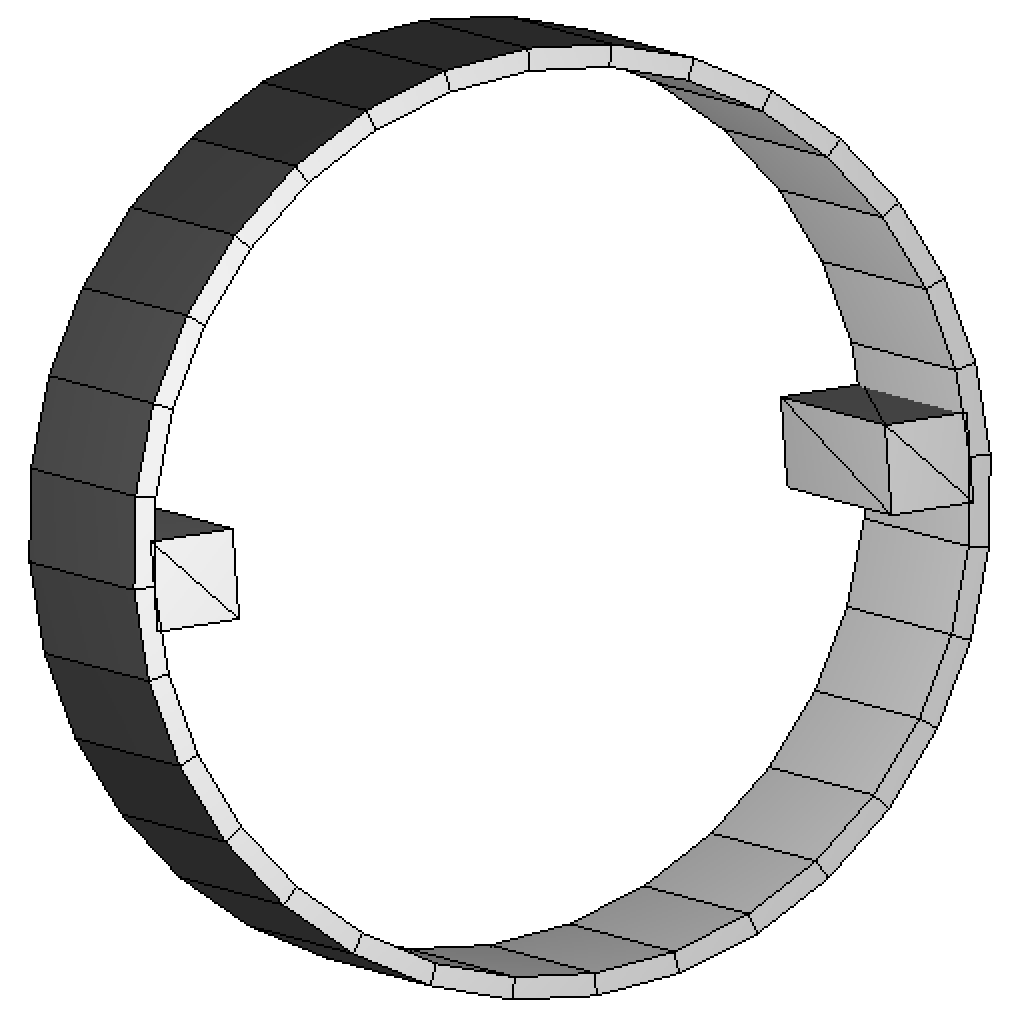
\includegraphics[width=0.22\textwidth]{drum0a}(b)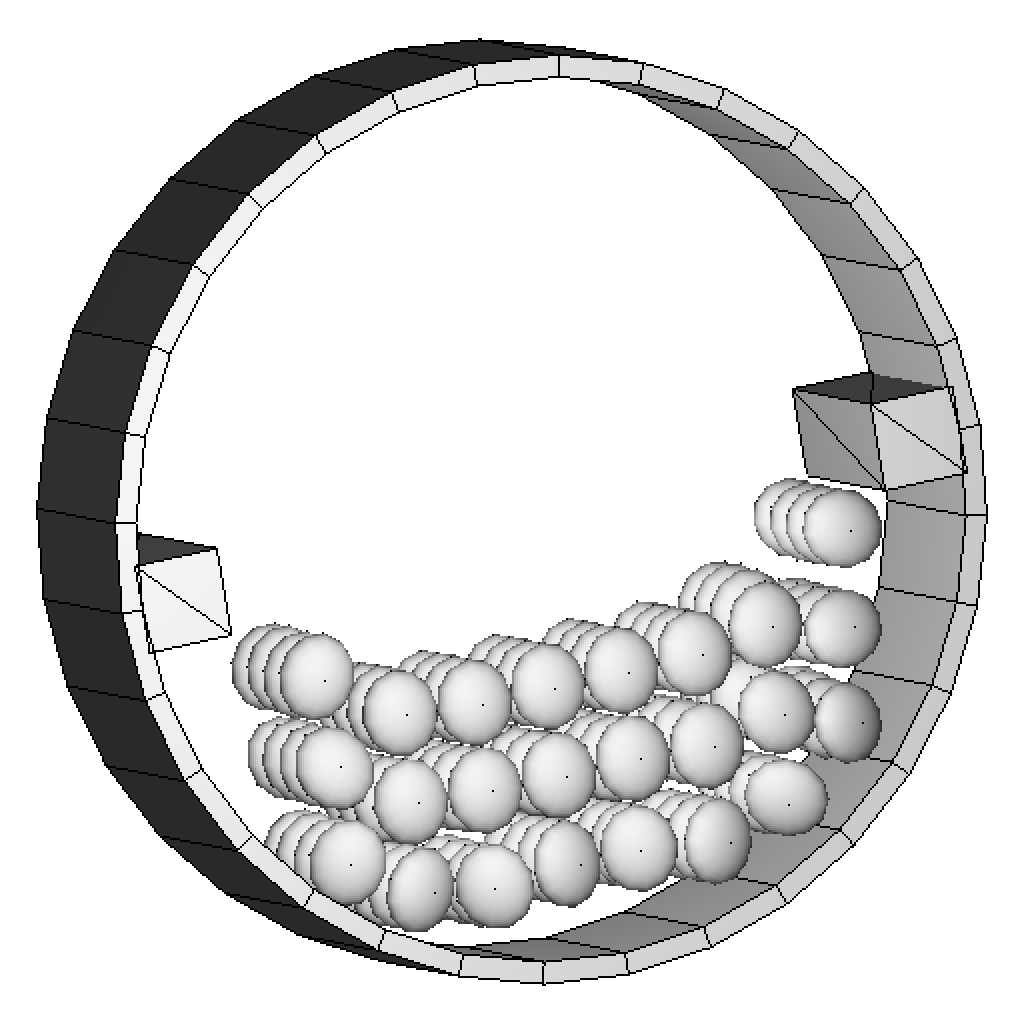
\includegraphics[width=0.22\textwidth]{drum0b}(c)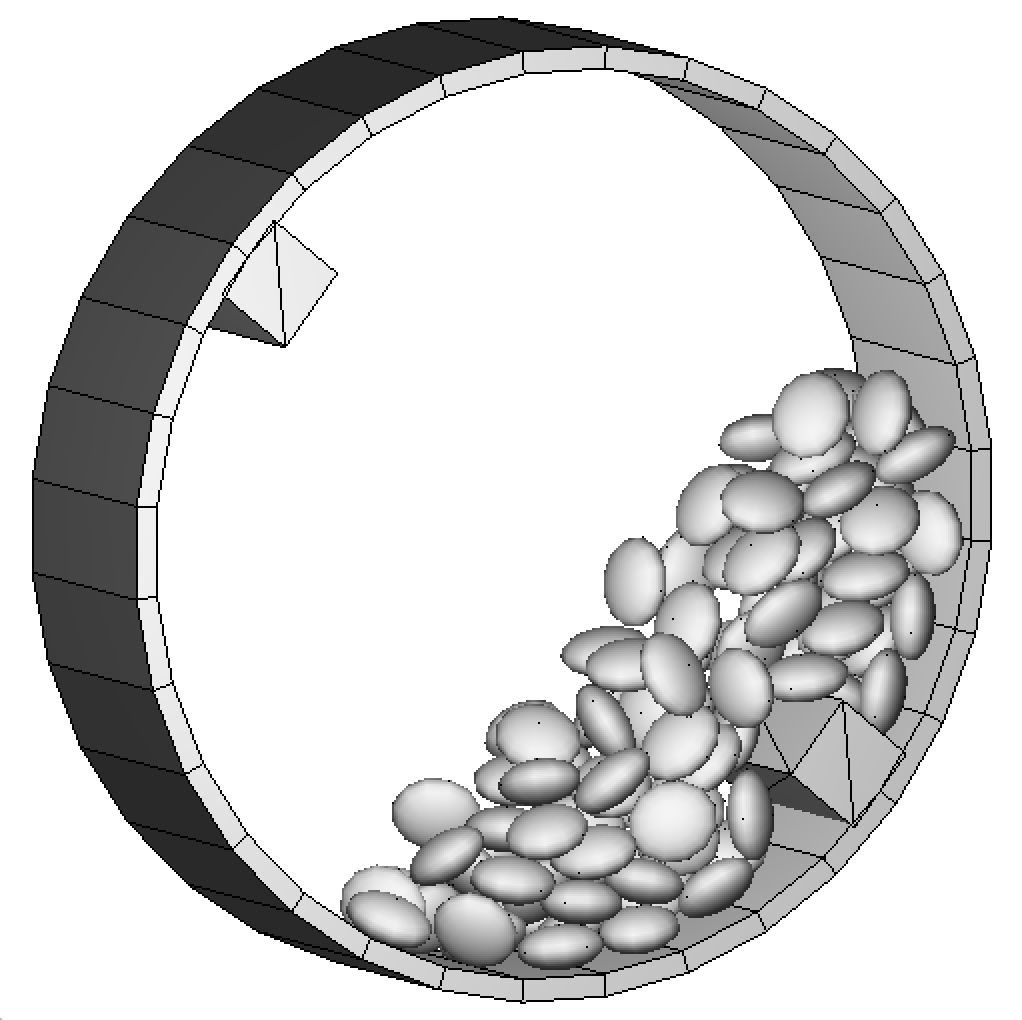
\includegraphics[width=0.22\textwidth]{drum0c}
\par\end{centering}
\caption{\label{fig:drum0}Rotating drum: drum geometry and simulation stages:
(a) empty drum, (b) dropping down the particles, (c) rotating the
drum.}
\end{figure}

\begin{figure}
\begin{centering}
(a)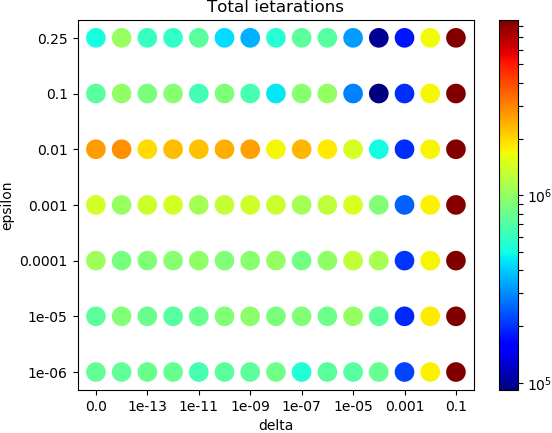
\includegraphics[width=0.33\textwidth]{dru100_RG_A0}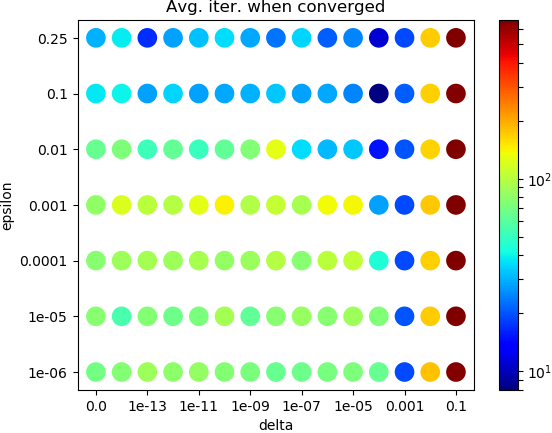
\includegraphics[width=0.33\textwidth]{dru100_RG_A1}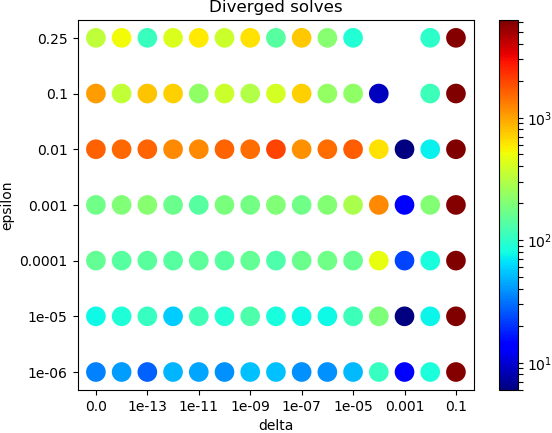
\includegraphics[width=0.33\textwidth]{dru100_RG_A2}
\par\end{centering}
\begin{centering}
(b)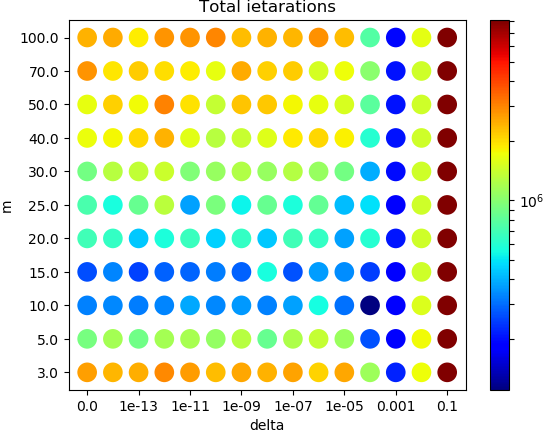
\includegraphics[width=0.33\textwidth]{dru100_RG_B0}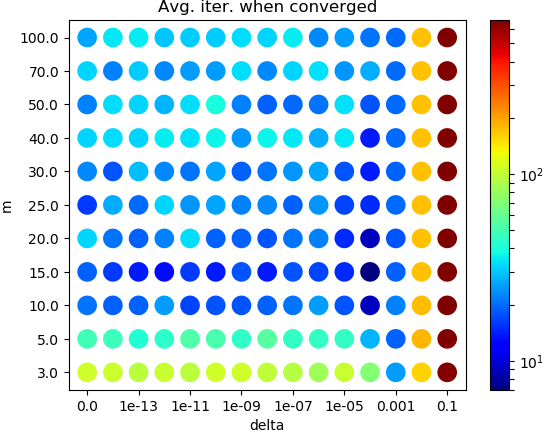
\includegraphics[width=0.33\textwidth]{dru100_RG_B1}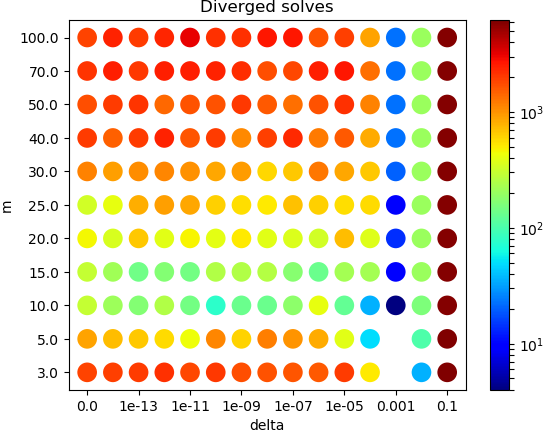
\includegraphics[width=0.33\textwidth]{dru100_RG_B2}
\par\end{centering}
\begin{centering}
(c)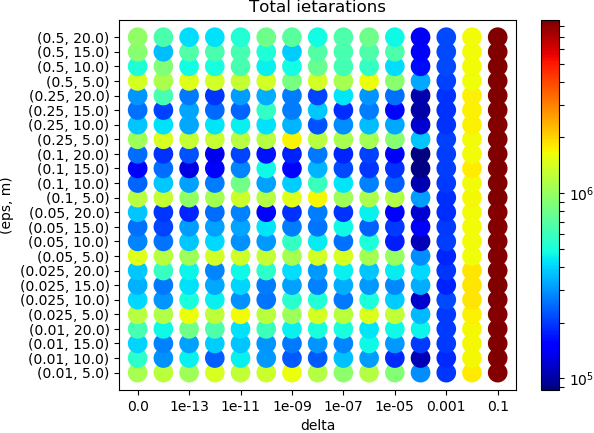
\includegraphics[width=0.33\textwidth]{dru100_RG_C0}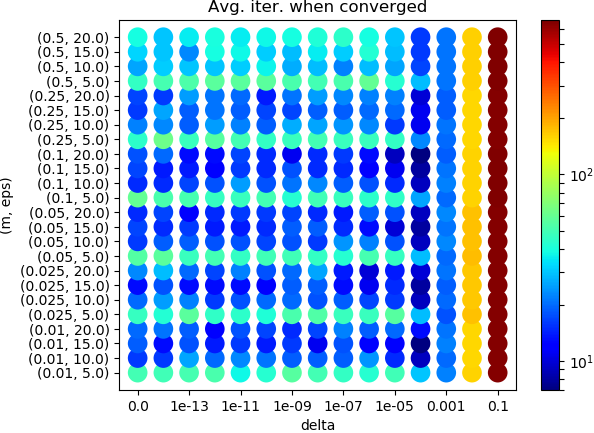
\includegraphics[width=0.33\textwidth]{dru100_RG_C1}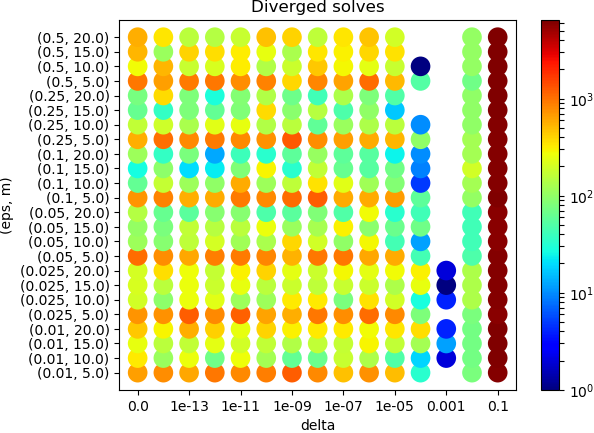
\includegraphics[width=0.33\textwidth]{dru100_RG_C2}
\par\end{centering}
\caption{\label{fig:drum1}Rotating drum ($N=100$, \emph{ell. rigid}): sensitivity
to the choice of $\delta$, $m$, and $\epsilon$; case (a) is for
$m=1000$ and varying $\delta,\epsilon$; case (b) is for $\epsilon=10^{-3}$
and varying $m,\delta;$ case (c) is for varying $\left(\epsilon,m\right)$
pairs and $\delta$; left to right we have: total iterations counts
across the entire simulation, average numbers of solver iterations
per time step when iterations are converged, and total (per simulation)
number of diverged Newton solver runs (when the Gauss-Seidel solver
was invoked upon reaching the iteration limit); missing dots in the
rightmost figures correspond to no cases of divergence.}
\end{figure}

\begin{figure}
\begin{centering}
(a)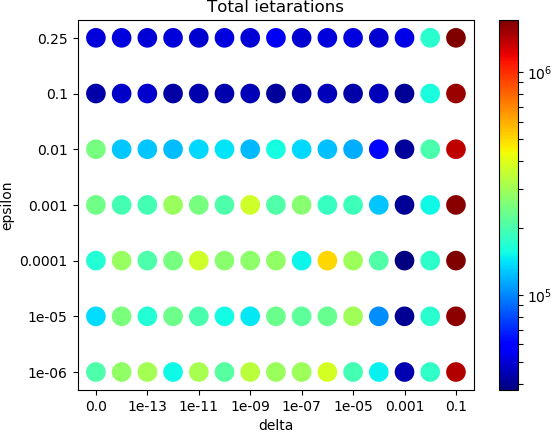
\includegraphics[width=0.33\textwidth]{dru100_PR_A0}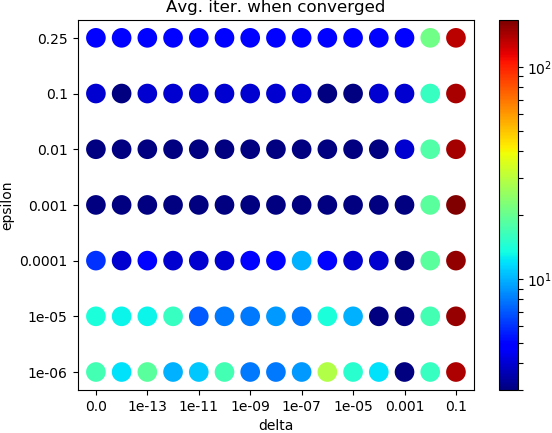
\includegraphics[width=0.33\textwidth]{dru100_PR_A1}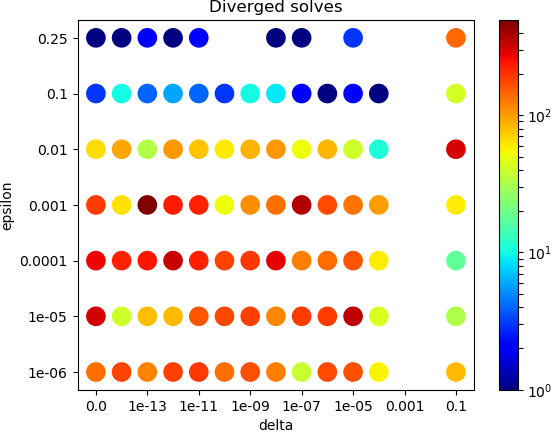
\includegraphics[width=0.33\textwidth]{dru100_PR_A2}
\par\end{centering}
\begin{centering}
(b)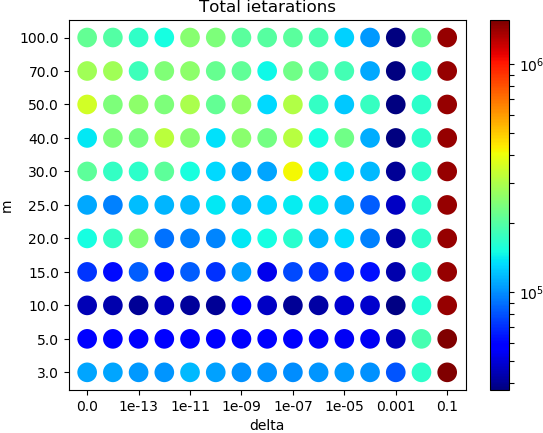
\includegraphics[width=0.33\textwidth]{dru100_PR_B0}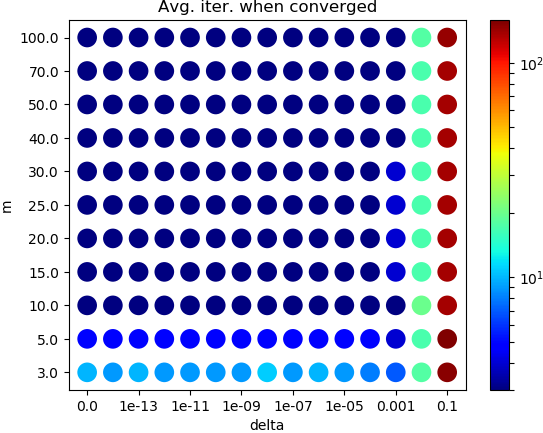
\includegraphics[width=0.33\textwidth]{dru100_PR_B1}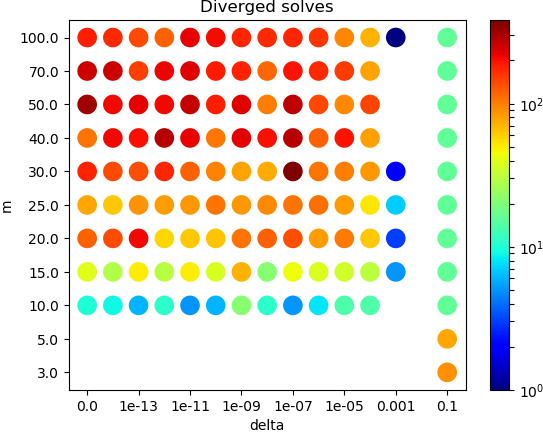
\includegraphics[width=0.33\textwidth]{dru100_PR_B2}
\par\end{centering}
\begin{centering}
(c)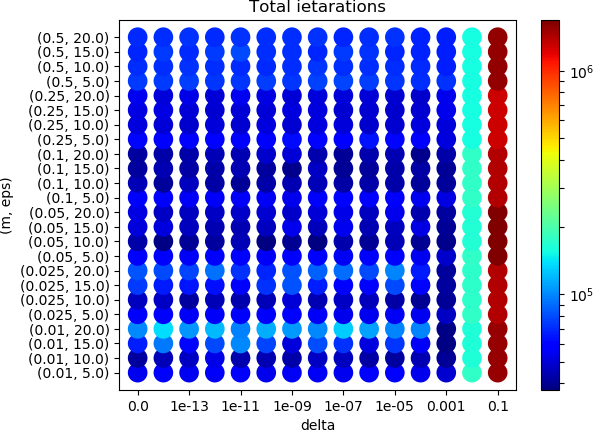
\includegraphics[width=0.33\textwidth]{dru100_PR_C0}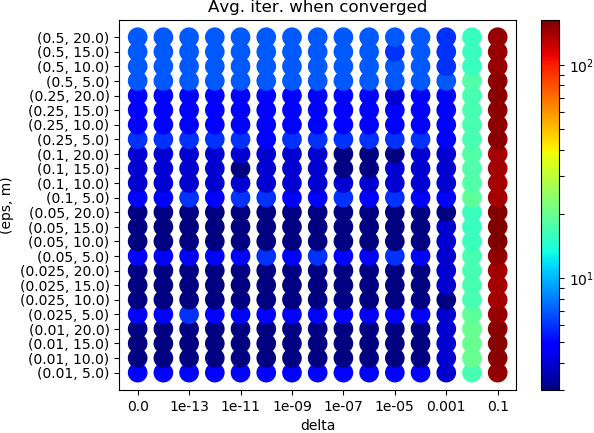
\includegraphics[width=0.33\textwidth]{dru100_PR_C1}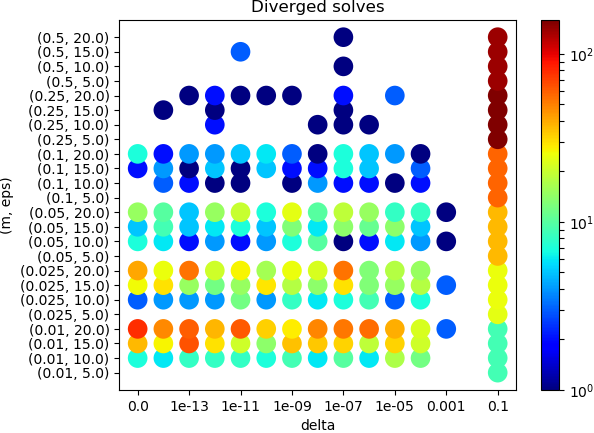
\includegraphics[width=0.33\textwidth]{dru100_PR_C2}
\par\end{centering}
\caption{\label{fig:drum2}Rotating drum ($N=100$, \emph{ell. defo}): sensitivity
to the choice of $\delta$, $m$, and $\epsilon$; sensitivity to
the choice of $\delta$, $m$, and $\epsilon$; case (a) is for $m=1000$
and varying $\delta,\epsilon$; case (b) is for $\epsilon=10^{-3}$
and varying $m,\delta;$ case (c) is for varying $\left(\epsilon,m\right)$
pairs and $\delta$; left to right we have: total iterations counts
across the entire simulation, average numbers of solver iterations
per time step when iterations are converged, and total (per simulation)
number of diverged Newton solver runs (when the Gauss-Seidel solver
was invoked upon reaching the iteration limit); missing dots in the
rightmost figures correspond to no cases of divergence.}
\end{figure}

\begin{figure}
\begin{centering}
(i)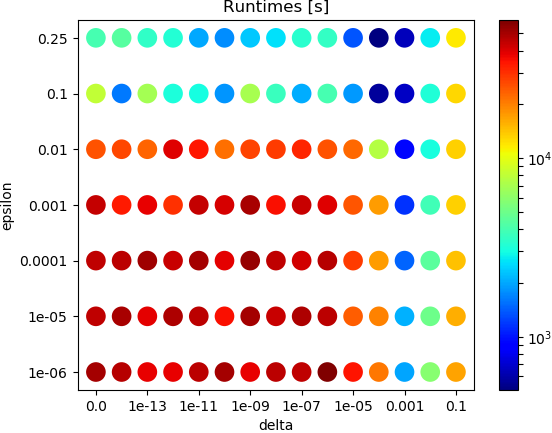
\includegraphics[width=0.33\textwidth]{dru100_RG_A_runtimes}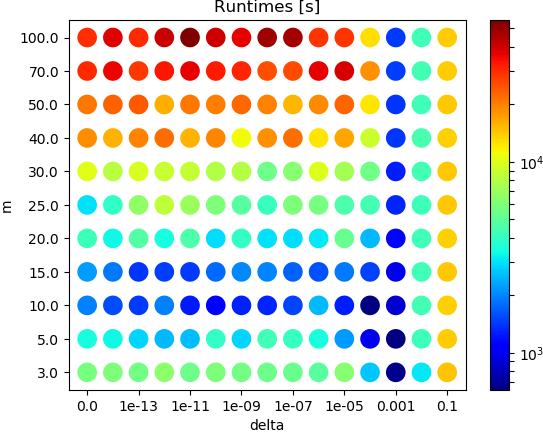
\includegraphics[width=0.33\textwidth]{dru100_RG_B_runtimes}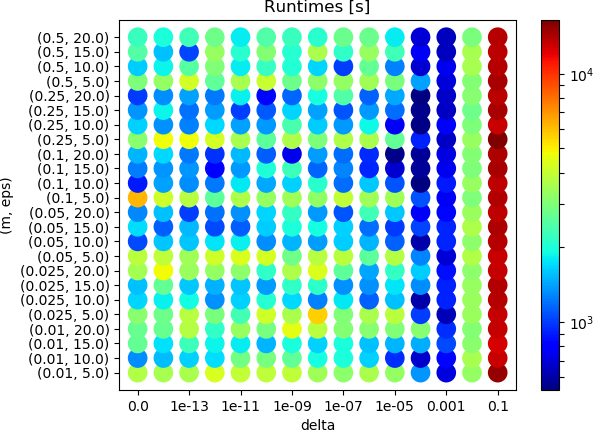
\includegraphics[width=0.33\textwidth]{dru100_RG_C_runtimes}
\par\end{centering}
\begin{centering}
(ii)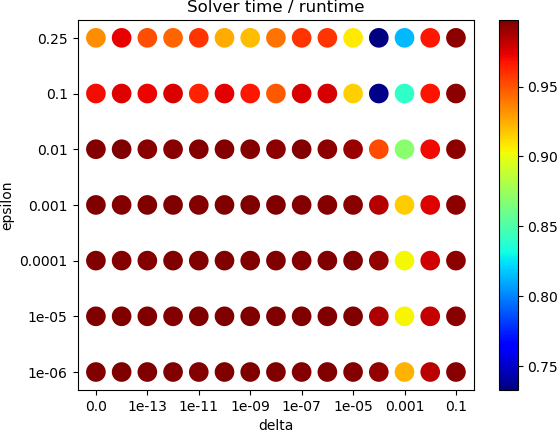
\includegraphics[width=0.33\textwidth]{dru100_RG_A_ratios}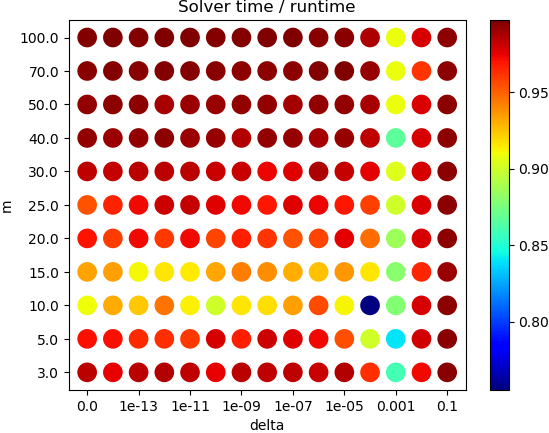
\includegraphics[width=0.33\textwidth]{dru100_RG_B_ratios}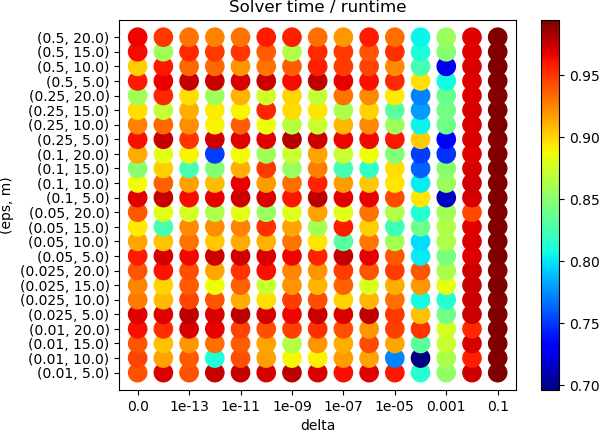
\includegraphics[width=0.33\textwidth]{dru100_RG_C_ratios}
\par\end{centering}
\caption{\label{fig:drum3}Rotating drum ($N=100$, \emph{ell. rigid}): runtimes
(i) and solver time to runtime ratios (ii); left to right figures
correspond to cases (a-c) in Figure \ref{fig:drum1}.}
\end{figure}

\begin{figure}
\begin{centering}
(i)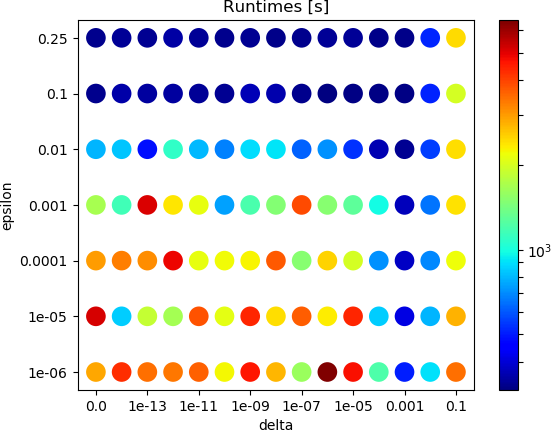
\includegraphics[width=0.33\textwidth]{dru100_PR_A_runtimes}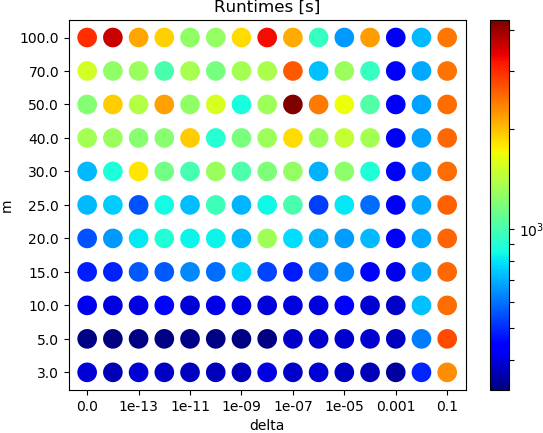
\includegraphics[width=0.33\textwidth]{dru100_PR_B_runtimes}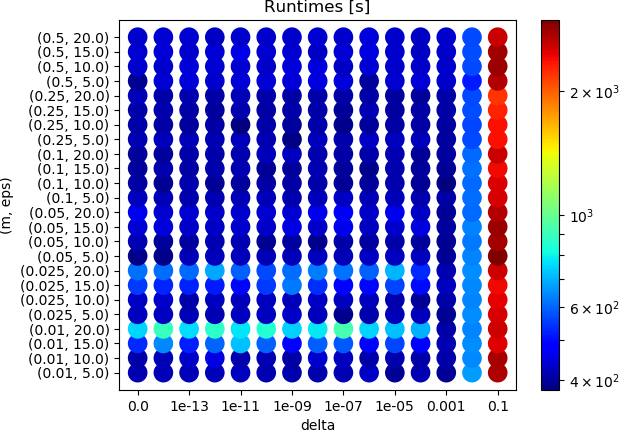
\includegraphics[width=0.33\textwidth]{dru100_PR_C_runtimes}
\par\end{centering}
\begin{centering}
(ii)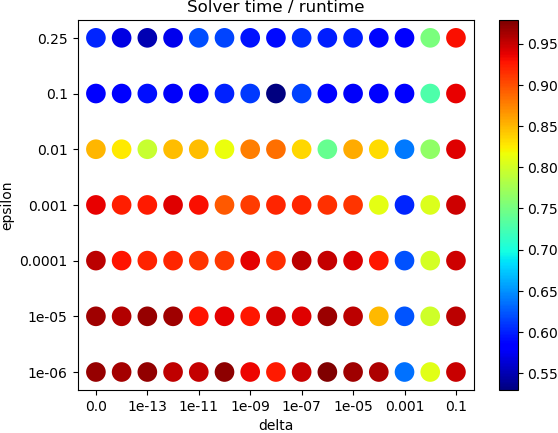
\includegraphics[width=0.33\textwidth]{dru100_PR_A_ratios}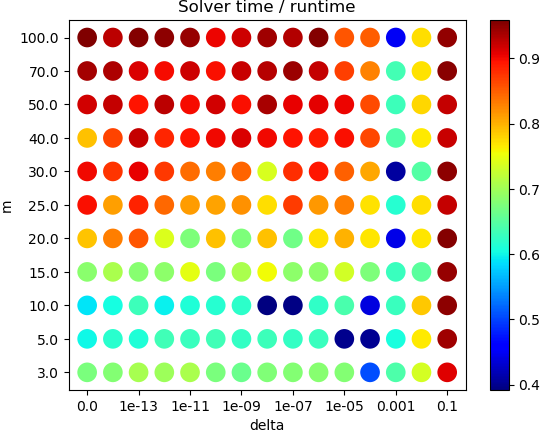
\includegraphics[width=0.33\textwidth]{dru100_PR_B_ratios}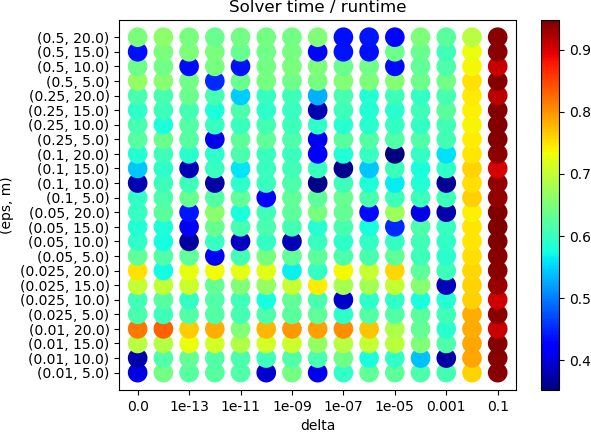
\includegraphics[width=0.33\textwidth]{dru100_PR_C_ratios}
\par\end{centering}
\caption{\label{fig:drum4}Rotating drum ($N=100$, \emph{ell. defo}): runtimes
(i) and solver time to runtime ratios (ii); left to right figures
correspond to cases (a-c) in Figure \ref{fig:drum2}.}
\end{figure}


\subsubsection{\label{subsec:absdelta}Sensitivity study: absolute $\delta$ values}

In this section the number of particles $N=100$. Figures \ref{fig:drum1}
and \ref{fig:drum2} depict sensitivity of the solver iteration counts
to the choice of $\delta$, $m$, and $\epsilon$. In case (a) the
linear solver iterations bound $m=1000$ and hence the linear solve
accuracy is dictated by the choice of $\epsilon$. In this case generally,
the more inexact the linear solve is the more robust the solver behavior
becomes: both the total and average numbers of iterations are lowest
for $\epsilon\in\left\{ 0.1,0.25\right\} $; for the rigid body case,
with $\delta=0.001$, the are no cases of divergence for these two
values of $\epsilon$; in the deformable case the entire vertical
strip at $\delta=0.001$ has this property and also there is no divergence
for several other combinations of $\delta$ and $\epsilon$. In case
(b) the absolute accuracy of the linear solver is kept constant at
$\epsilon=0.001$ while the number of linear solver iterations $m$
is varied. In this case it is also clear that inexact solves are favorable,
with lowest total and average numbers of iterations for $m\in\left\{ 10,15\right\} $
for both the rigid and deformable case. There are no solver failures
for $\delta=0.001$ and $m\in\left\{ 3,5\right\} $ in the rigid case,
while a significantly larger set of parameters $m\in\left\{ 3,5\right\} $
\textbf{or} $\delta\in\left\{ 0.001,0.01\right\} $ is free of solver
divergence (with an exception of one data point). Quite clearly -
inexact linear solves are favored. Case (c) samples sensitivity in
the space of various $\left(\epsilon,m\right)$ choices and the varying
regularization parameter $\delta$. In the rigid case (Figure \ref{fig:drum1}
(c), right) it is seen that the entire $\delta=0.001$ is nearly free
of solver divergence; a significantly large parameter space has this
property in the deformable case (Figure \ref{fig:drum2} (c), right).
We can also see that for the rigid case the average number of iterations
per time step is in the range 10-100, while in the deformable case
it is in the range 1-10. Consequently, there is a similar correspondence
between the total number of iterations (scaled up by 10000: the number
of time steps).

The runtimes and solver time to runtime ratios are depicted in Figure
\ref{fig:drum3} and \ref{fig:drum4}. Shortest runtimes and lowest
timing ratios correspond to the same parameter set choices as those
transpiring in Figures \ref{fig:drum1} and \ref{fig:drum2}. For
the rigid body case, the choice of (0.0001, 0.25, 15) for the $\left(\delta,\epsilon,m\right)$
triad produces the shortest total runtime of 525s (with zero solver
failures). For the pseudo-rigid kinematic case, the choice of (1E-13,
0.25, 20) for the $\left(\delta,\epsilon,m\right)$ triad produces
the shortest total runtime of 356s (with zero solver failures). These
runtimes are well comparable with those produced by the Gauss-Seidel
solver based runs and reported in Table \ref{tab:drum1}.

\begin{table}
\begin{centering}
\begin{tabular}{|c|c|c|c|c|c|c|c|c|}
\cline{2-9} 
\multicolumn{1}{c|}{} & \multicolumn{4}{c|}{Newton solver based} & \multicolumn{4}{c|}{Gauss-Seidel solver based}\tabularnewline
\cline{2-9} 
\multicolumn{1}{c|}{} & runtime & ratio & it/step & divs & runtime & ratio & it/step & divs\tabularnewline
\hline 
ell. rigid & 525s & 0.78 & 10 & 0 & 495s & 0.85 & 112 & 20\tabularnewline
\hline 
ell. defo & 356s & 0.64 & 5 & 0 & 482s & 0.45 & 18 & 0\tabularnewline
\hline 
sph. rigid &  &  &  &  & 462s & 0.96 & 174 & 330\tabularnewline
\hline 
sph. defo &  &  &  &  & 64s & 0.64 & 21 & 0\tabularnewline
\hline 
\end{tabular}
\par\end{centering}
\caption{\label{tab:drum1}Rotating drum $\left(N=100\right)$: comparison
of solution statistics for $\left(\delta,\epsilon,m\right)$ choice
of (0.0001, 0.25, 15) for the rigid body case and (1E-13, 0.25, 20)
for the deformable body case; respective columns stand for total runtime
in seconds (runtime), solver time to runtime ratio (ratio), average
number of iterations per step when converged (it/step), and number
of diverged steps.}
\end{table}


\subsubsection{\label{subsec:reldelta}Sensitivity study: relative $\delta$ values}

The choice of the regularization parameter $\delta$ as an absolute
value may not always be practical. For simulation setups with many
particles it may not be possible to run many large scale tests in
order to tune $\delta.$ It may be more practical to study solver
performance on a smaller example, just like in this section, and then
attempt to reuse the set of recommended parameters for larger scale
runs. This is why investigating a choice of $\delta$ as relative
to a norm of the $\mathbf{W}$ operator (\ref{eq:W}) is relevant.
Three such choices are investigated here:

\[
\delta_{1}=\delta\cdot\min_{i}W_{ii}\text{ or }\delta_{1}=\delta\cdot\underset{i}{\text{avg}}W_{ii}\text{ or }\delta_{1}=\delta\cdot\max_{i}W_{ii}
\]
where $W_{ii}$ are the diagonal entries of $\mathbf{W}$. Consequently,
$\delta_{1}$ is used in line 2b of Algorithm \ref{alg:PQN} instead
of $\delta$. The same studies as in Section \ref{subsec:absdelta}
are repeated in the current case. The results are juxtaposed in Figures
\ref{fig:drum1-minWii}-\ref{fig:drum2-maxWii}.

\begin{figure}
\begin{centering}
(a)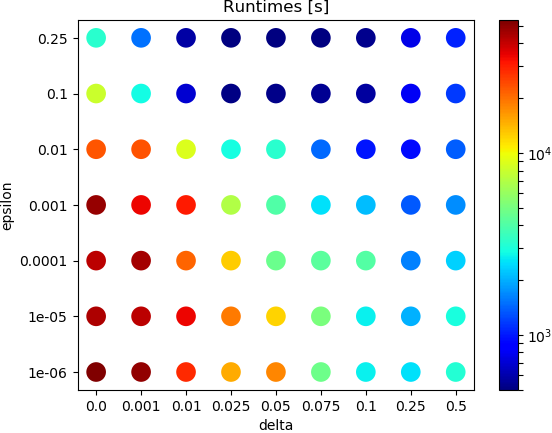
\includegraphics[width=0.33\textwidth]{dru100_RG_A_minWii_runtimes}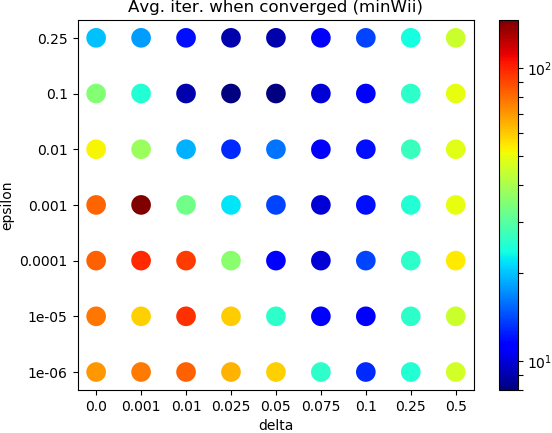
\includegraphics[width=0.33\textwidth]{dru100_RG_A1_minWii}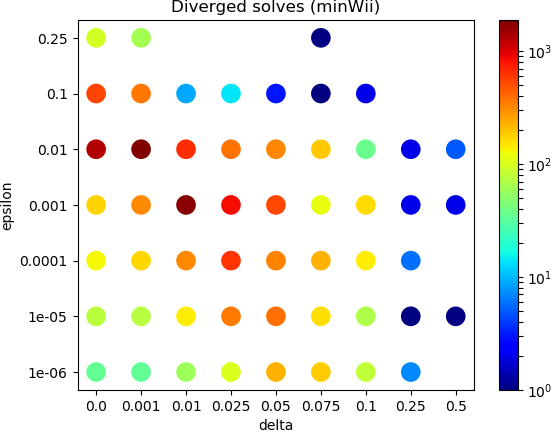
\includegraphics[width=0.33\textwidth]{dru100_RG_A2_minWii}
\par\end{centering}
\begin{centering}
(b)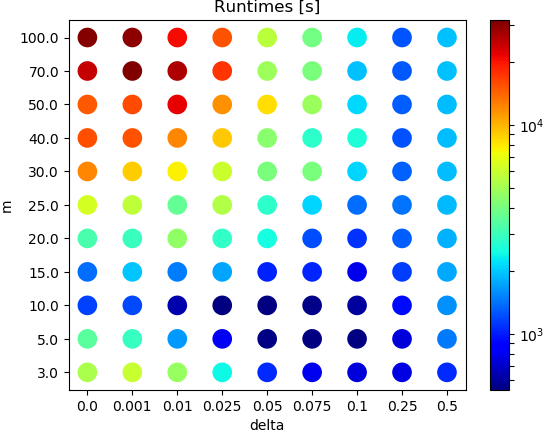
\includegraphics[width=0.33\textwidth]{dru100_RG_B_minWii_runtimes}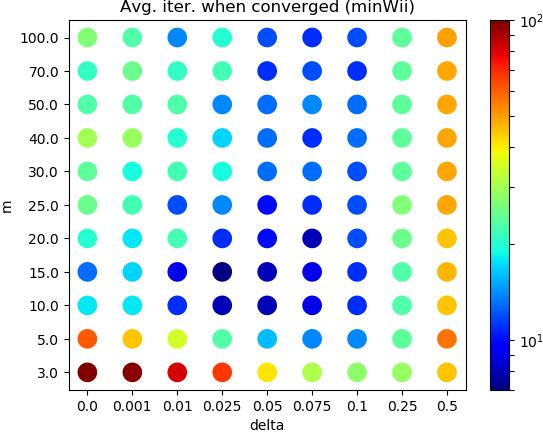
\includegraphics[width=0.33\textwidth]{dru100_RG_B1_minWii}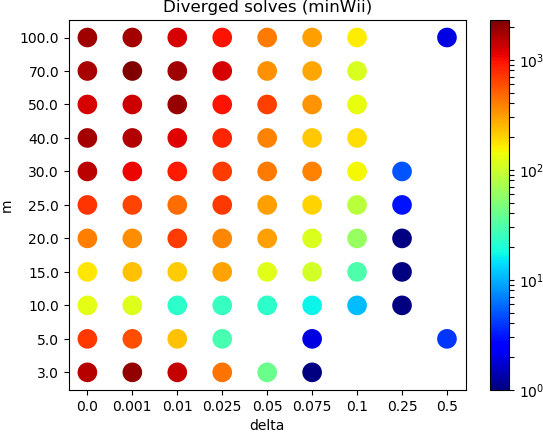
\includegraphics[width=0.33\textwidth]{dru100_RG_B2_minWii}
\par\end{centering}
\begin{centering}
(c)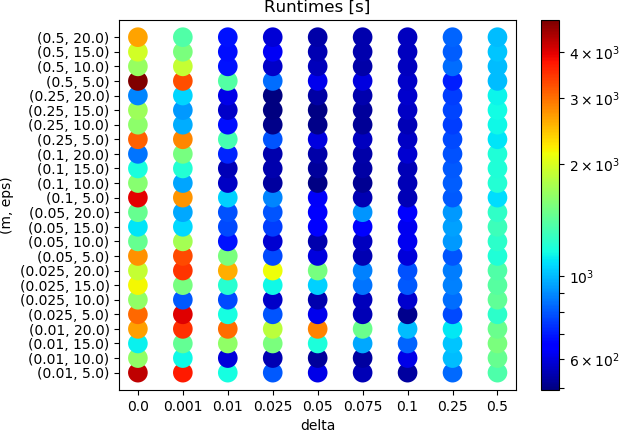
\includegraphics[width=0.33\textwidth]{dru100_RG_C_minWii_runtimes}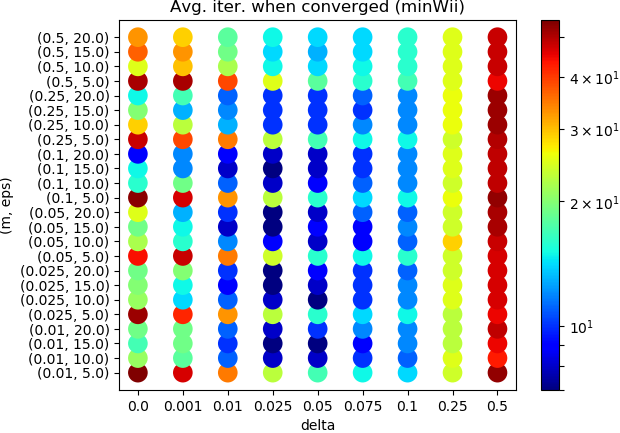
\includegraphics[width=0.33\textwidth]{dru100_RG_C1_minWii}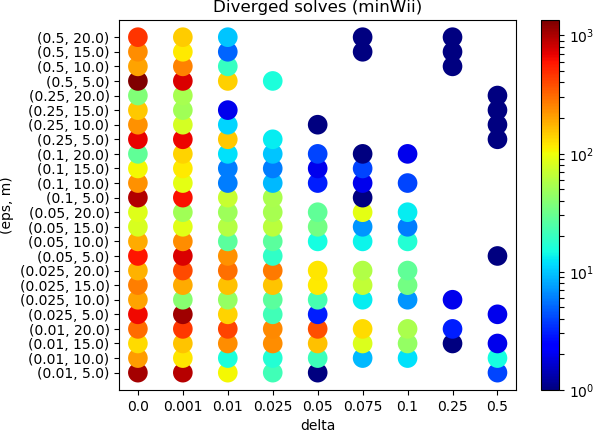
\includegraphics[width=0.33\textwidth]{dru100_RG_C2_minWii}
\par\end{centering}
\caption{\label{fig:drum1-minWii}Rotating drum ($N=100$, \emph{ell. rigid},
$\delta_{1}=\delta\cdot\min_{i}W_{ii}$): sensitivity to the choice
of $\delta$, $m$, and $\epsilon$; case (a) is for $m=1000$ and
varying $\delta,\epsilon$; case (b) is for $\epsilon=10^{-3}$ and
varying $m,\delta;$ case (c) is for varying $\left(\epsilon,m\right)$
pairs and $\delta$; left to right we have: total runtimes, average
numbers of solver iterations per time step when iterations are converged,
and total (per simulation) number of diverged Newton solver runs (when
the Gauss-Seidel solver was invoked upon reaching the iteration limit);
missing dots in the rightmost figures correspond to no cases of divergence.}
\end{figure}

\begin{figure}
\begin{centering}
(a)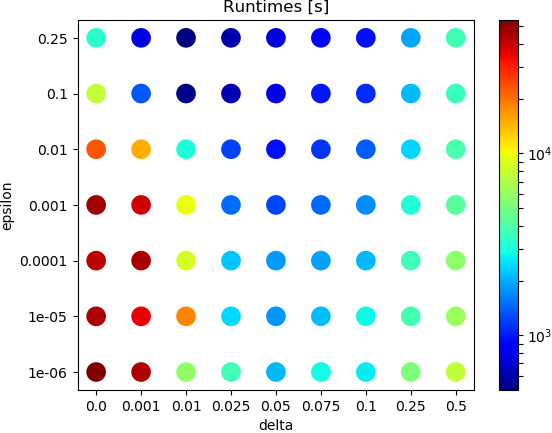
\includegraphics[width=0.33\textwidth]{dru100_RG_A_avgWii_runtimes}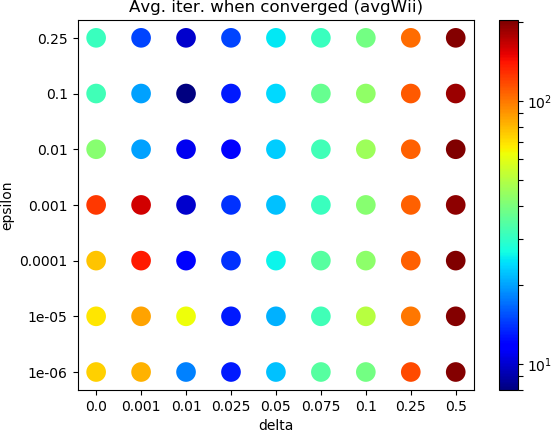
\includegraphics[width=0.33\textwidth]{dru100_RG_A1_avgWii}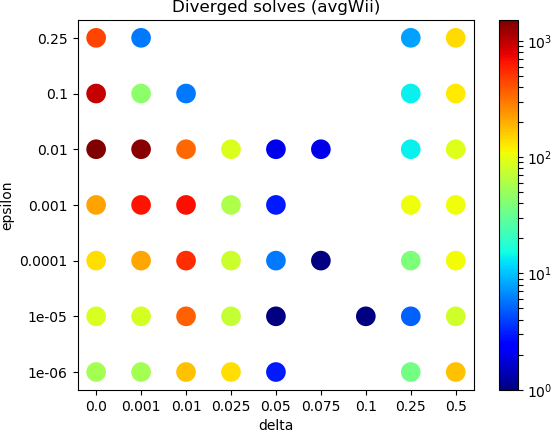
\includegraphics[width=0.33\textwidth]{dru100_RG_A2_avgWii}
\par\end{centering}
\begin{centering}
(b)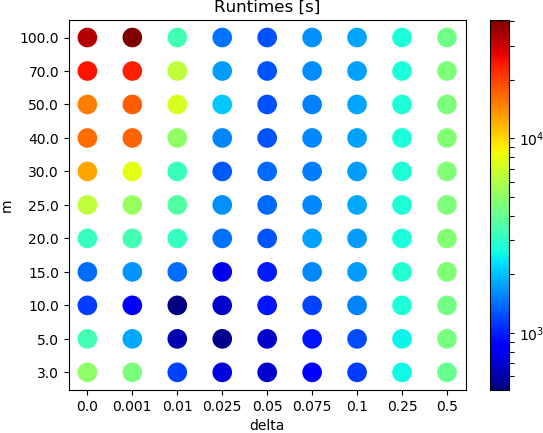
\includegraphics[width=0.33\textwidth]{dru100_RG_B_avgWii_runtimes}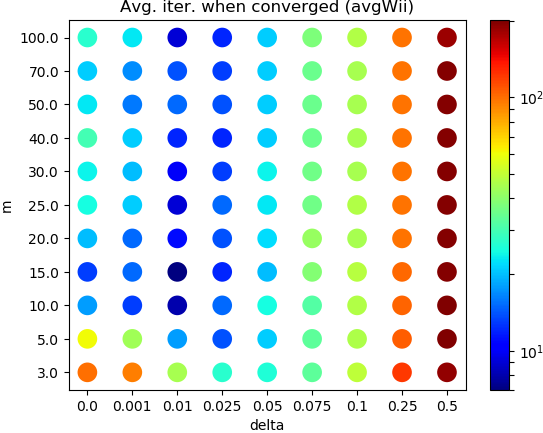
\includegraphics[width=0.33\textwidth]{dru100_RG_B1_avgWii}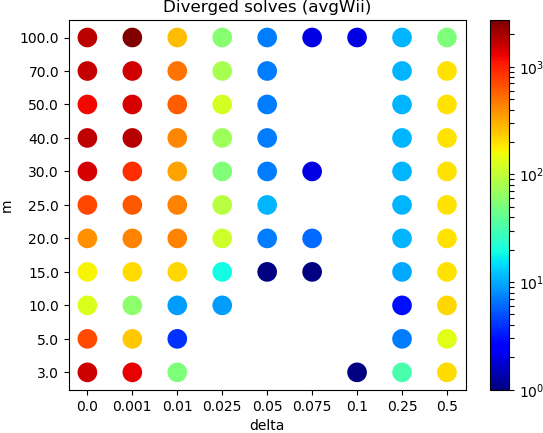
\includegraphics[width=0.33\textwidth]{dru100_RG_B2_avgWii}
\par\end{centering}
\begin{centering}
(c)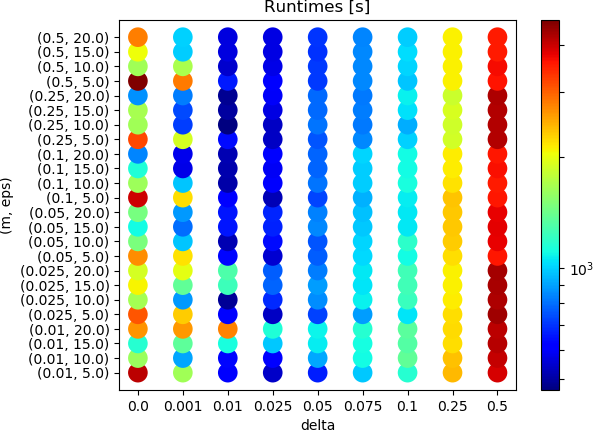
\includegraphics[width=0.33\textwidth]{dru100_RG_C_avgWii_runtimes}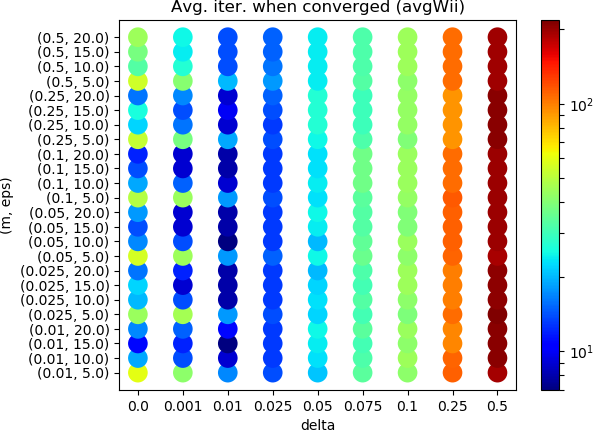
\includegraphics[width=0.33\textwidth]{dru100_RG_C1_avgWii}\includegraphics[width=0.33\textwidth]{dru100_RG_C2_avgWii}
\par\end{centering}
\caption{\label{fig:drum1-avgWii}Rotating drum ($N=100$, \emph{ell. rigid},
$\delta_{1}=\delta\cdot\protect\underset{i}{\text{avg}}W_{ii}$):
sensitivity to the choice of $\delta$, $m$, and $\epsilon$; case
(a) is for $m=1000$ and varying $\delta,\epsilon$; case (b) is for
$\epsilon=10^{-3}$ and varying $m,\delta;$ case (c) is for varying
$\left(\epsilon,m\right)$ pairs and $\delta$; left to right we have:
total runtimes, average numbers of solver iterations per time step
when iterations are converged, and total (per simulation) number of
diverged Newton solver runs (when the Gauss-Seidel solver was invoked
upon reaching the iteration limit); missing dots in the rightmost
figures correspond to no cases of divergence.}
\end{figure}

\begin{figure}
\begin{centering}
(a)\includegraphics[width=0.33\textwidth]{dru100_RG_A_maxWii_runtimes}\includegraphics[width=0.33\textwidth]{dru100_RG_A1_maxWii}\includegraphics[width=0.33\textwidth]{dru100_RG_A2_maxWii}
\par\end{centering}
\begin{centering}
(b)\includegraphics[width=0.33\textwidth]{dru100_RG_B_maxWii_runtimes}\includegraphics[width=0.33\textwidth]{dru100_RG_B1_maxWii}\includegraphics[width=0.33\textwidth]{dru100_RG_B2_maxWii}
\par\end{centering}
\begin{centering}
(c)\includegraphics[width=0.33\textwidth]{dru100_RG_C_maxWii_runtimes}\includegraphics[width=0.33\textwidth]{dru100_RG_C1_maxWii}\includegraphics[width=0.33\textwidth]{dru100_RG_C2_maxWii}
\par\end{centering}
\caption{\label{fig:drum1-maxWii}Rotating drum ($N=100$, \emph{ell. rigid},
$\delta_{1}=\delta\cdot\max_{i}W_{ii}$): sensitivity to the choice
of $\delta$, $m$, and $\epsilon$; case (a) is for $m=1000$ and
varying $\delta,\epsilon$; case (b) is for $\epsilon=10^{-3}$ and
varying $m,\delta;$ case (c) is for varying $\left(\epsilon,m\right)$
pairs and $\delta$; left to right we have: total runtimes, average
numbers of solver iterations per time step when iterations are converged,
and total (per simulation) number of diverged Newton solver runs (when
the Gauss-Seidel solver was invoked upon reaching the iteration limit);
missing dots in the rightmost figures correspond to no cases of divergence.}
\end{figure}

\begin{figure}
\begin{centering}
(a)\includegraphics[width=0.33\textwidth]{dru100_PR_A_minWii_runtimes}\includegraphics[width=0.33\textwidth]{dru100_PR_A1_minWii}\includegraphics[width=0.33\textwidth]{dru100_PR_A2_minWii}
\par\end{centering}
\begin{centering}
(b)\includegraphics[width=0.33\textwidth]{dru100_PR_B_minWii_runtimes}\includegraphics[width=0.33\textwidth]{dru100_PR_B1_minWii}\includegraphics[width=0.33\textwidth]{dru100_PR_B2_minWii}
\par\end{centering}
\begin{centering}
(c)\includegraphics[width=0.33\textwidth]{dru100_PR_C_minWii_runtimes}\includegraphics[width=0.33\textwidth]{dru100_PR_C1_minWii}\includegraphics[width=0.33\textwidth]{dru100_PR_C2_minWii}
\par\end{centering}
\caption{\label{fig:drum2-minWii}Rotating drum ($N=100$, \emph{ell. defo},
$\delta_{1}=\delta\cdot\min_{i}W_{ii}$): sensitivity to the choice
of $\delta$, $m$, and $\epsilon$; case (a) is for $m=1000$ and
varying $\delta,\epsilon$; case (b) is for $\epsilon=10^{-3}$ and
varying $m,\delta;$ case (c) is for varying $\left(\epsilon,m\right)$
pairs and $\delta$; left to right we have: total runtimes, average
numbers of solver iterations per time step when iterations are converged,
and total (per simulation) number of diverged Newton solver runs (when
the Gauss-Seidel solver was invoked upon reaching the iteration limit);
missing dots in the rightmost figures correspond to no cases of divergence.}
\end{figure}

\begin{figure}
\begin{centering}
(a)\includegraphics[width=0.33\textwidth]{dru100_PR_A_avgWii_runtimes}\includegraphics[width=0.33\textwidth]{dru100_PR_A1_avgWii}\includegraphics[width=0.33\textwidth]{dru100_PR_A2_avgWii}
\par\end{centering}
\begin{centering}
(b)\includegraphics[width=0.33\textwidth]{dru100_PR_B_avgWii_runtimes}\includegraphics[width=0.33\textwidth]{dru100_PR_B1_avgWii}\includegraphics[width=0.33\textwidth]{dru100_PR_B2_avgWii}
\par\end{centering}
\begin{centering}
(c)\includegraphics[width=0.33\textwidth]{dru100_PR_C_avgWii_runtimes}\includegraphics[width=0.33\textwidth]{dru100_PR_C1_avgWii}\includegraphics[width=0.33\textwidth]{dru100_PR_C2_avgWii}
\par\end{centering}
\caption{\label{fig:drum2-avgWii}Rotating drum ($N=100$, \emph{ell. defo},
$\delta_{1}=\delta\cdot\protect\underset{i}{\text{avg}}W_{ii}$):
sensitivity to the choice of $\delta$, $m$, and $\epsilon$; case
(a) is for $m=1000$ and varying $\delta,\epsilon$; case (b) is for
$\epsilon=10^{-3}$ and varying $m,\delta;$ case (c) is for varying
$\left(\epsilon,m\right)$ pairs and $\delta$; left to right we have:
total runtimes, average numbers of solver iterations per time step
when iterations are converged, and total (per simulation) number of
diverged Newton solver runs (when the Gauss-Seidel solver was invoked
upon reaching the iteration limit); missing dots in the rightmost
figures correspond to no cases of divergence.}
\end{figure}

\begin{figure}
\begin{centering}
(a)\includegraphics[width=0.33\textwidth]{dru100_PR_A_maxWii_runtimes}\includegraphics[width=0.33\textwidth]{dru100_PR_A1_maxWii}\includegraphics[width=0.33\textwidth]{dru100_PR_A2_maxWii}
\par\end{centering}
\begin{centering}
(b)\includegraphics[width=0.33\textwidth]{dru100_PR_B_maxWii_runtimes}\includegraphics[width=0.33\textwidth]{dru100_PR_B1_maxWii}\includegraphics[width=0.33\textwidth]{dru100_PR_B2_maxWii}
\par\end{centering}
\begin{centering}
(c)\includegraphics[width=0.33\textwidth]{dru100_PR_C_maxWii_runtimes}\includegraphics[width=0.33\textwidth]{dru100_PR_C1_maxWii}\includegraphics[width=0.33\textwidth]{dru100_PR_C2_maxWii}
\par\end{centering}
\caption{\label{fig:drum2-maxWii}Rotating drum ($N=100$, \emph{ell. defo},
$\delta_{1}=\delta\cdot\max_{i}W_{ii}$): sensitivity to the choice
of $\delta$, $m$, and $\epsilon$; case (a) is for $m=1000$ and
varying $\delta,\epsilon$; case (b) is for $\epsilon=10^{-3}$ and
varying $m,\delta;$ case (c) is for varying $\left(\epsilon,m\right)$
pairs and $\delta$; left to right we have: total runtimes, average
numbers of solver iterations per time step when iterations are converged,
and total (per simulation) number of diverged Newton solver runs (when
the Gauss-Seidel solver was invoked upon reaching the iteration limit);
missing dots in the rightmost figures correspond to no cases of divergence.}
\end{figure}

By browsing Figures \ref{fig:drum1-minWii}-\ref{fig:drum2-maxWii}
we notice that cases of fully robust runs (without divergence) are
significantly more common when the choice of $\delta_{1}$ is relative
to $\mathbf{W}$. As we move from the $\min W_{ii}$ norm, through
the average $W_{ii}$ norm, to the $\max W_{ii}$ norm, the region
of no solver failures gradually moves from right to left \textendash{}
within the unchanging range of the relative span of $\delta$. This
reflects the fact that the absolute range of values of $\delta_{1}$
for which no failures occur becomes better represented (within the
chosen and fixed range of $\delta$) as we shift between $\min W_{ii}\rightarrow\text{avg}W_{ii}\rightarrow\max W_{ii}$.
Perhaps it does not matter which of those norms we use as long as
in our investigation of an optimum value of $\delta$ we cover a sufficient
range. We can also see, that for rigid ellipsoids this range is narrower
when compared with the deformable counterpart: the no failure zone
is significantly broader in case of pseudo-rigid ellipsoids. This
corresponds to the fact that it is easier to resolve contact reactions
with the extra kinematic freedom allowing for the particles themselves
to deform.

In all of the Figures \ref{fig:drum1-minWii}-\ref{fig:drum2-maxWii}
the areas of shortest runtimes do not necessarily strictly correspond
to the areas of no solver failure. There are overlap zones where both
properties meet, but in general shortest runtimes occur in areas where
both, the average number of solver iterations per time step, and the
number of solver failures, are simultaneously low. Having only few
instances of a fallback on the Gauss-Seidel solver during the entire
simulation does not significantly affect the runtime. Nonetheless,
it is possible to select parameter sets for which there are no solver
failures and the runtime is short. For the rigid body case, the choice
of $\left(0.01_{\text{avg}W_{ii}},0.25,10\right)$ for the $\left(\delta_{\text{avg}W_{ii}},\epsilon,m\right)$
triad produces the shortest total runtime of 467s (with zero solver
failures). For the pseudo-rigid kinematic case, the choice of $\left(0.01_{\text{avg}W_{ii}},0.01,5\right)$
for the $\left(\delta_{\text{avg}W_{ii}},\epsilon,m\right)$ triad
produces the shortest total runtime of 352s (with zero solver failures).
These runtimes are well comparable with those produced by the Gauss-Seidel
solver based runs and reported in Table \ref{tab:drum1-reldelta}.
Table \ref{tab:drum1-normtimes} juxtaposes shortest runtimes for
all three choices of the relative $\delta$ norms.

\begin{table}
\begin{centering}
\begin{tabular}{|c|c|c|c|c|c|c|c|c|}
\cline{2-9} 
\multicolumn{1}{c|}{} & \multicolumn{4}{c|}{Newton solver based} & \multicolumn{4}{c|}{Gauss-Seidel solver based}\tabularnewline
\cline{2-9} 
\multicolumn{1}{c|}{} & runtime & ratio & it/step & divs & runtime & ratio & it/step & divs\tabularnewline
\hline 
ell. rigid & 467s & 0.77 & 9 & 0 & 495s & 0.85 & 112 & 20\tabularnewline
\hline 
ell. defo & 352s & 0.65 & 5 & 0 & 482s & 0.45 & 18 & 0\tabularnewline
\hline 
sph. rigid &  &  &  &  & 462s & 0.96 & 174 & 330\tabularnewline
\hline 
sph. defo &  &  &  &  & 64s & 0.64 & 21 & 0\tabularnewline
\hline 
\end{tabular}
\par\end{centering}
\caption{\label{tab:drum1-reldelta}Rotating drum $\left(N=100\right)$: comparison
of solution statistics for $\left(\delta,\epsilon,m\right)$ choice
of $\left(0.01_{\text{avg}W_{ii}},0.25,10\right)$ for the rigid body
case and $\left(0.01_{\text{avg}W_{ii}},0.01,5\right)$ for the deformable
body case; respective columns stand for total runtime in seconds (runtime),
solver time to runtime ratio (ratio), average number of iterations
per step when converged (it/step), and number of diverged steps.}
\end{table}

\begin{table}
\begin{centering}
\begin{tabular}{|c|c|c|c|c|c|}
\cline{3-6} 
\multicolumn{2}{c|}{} & runtime & $\delta$ & $\epsilon$ & $m$\tabularnewline
\hline 
\multirow{3}{*}{rigid} & $\min W_{ii}$ & 495s & 0.025 & 0.25 & 15\tabularnewline
\cline{2-6} 
 & $\text{avg}W_{ii}$ & 467s & 0.01 & 0.25 & 10\tabularnewline
\cline{2-6} 
 & $\max$$W_{ii}$ & 525s & 0.01 & 0.25 & 20\tabularnewline
\hline 
\multirow{3}{*}{defo} & $\min W_{ii}$ & 378s & 0.1 & 0.1 & 20\tabularnewline
\cline{2-6} 
 & $\text{avg}W_{ii}$ & 352s & 0.01 & 0.01 & 5\tabularnewline
\cline{2-6} 
 & $\max$$W_{ii}$ & 385s & 0.01 & 0.05 & 10\tabularnewline
\hline 
\end{tabular}
\par\end{centering}
\caption{\label{tab:drum1-normtimes}Rotating drum $\left(N=100\right)$: juxtaposition
of shortest runtimes and parameter choices for all three relative
$\delta$ norms.}

\end{table}


\subsubsection{Sensitivity study: material density vs. relative $\delta$ choices}

Small scale simulations like in Sections \ref{subsec:absdelta} and
\ref{subsec:reldelta} are suitable for exploring and tuning solver
parameters. Nonetheless, in case of large scale simulations, such
direct tuning would not be practical - consuming too much resources
and time. When modifying aspects of a simulation setup (e.g. material
parameters, geometrical dimensions, number of particles) it is useful
to have an orientation whether a set of optimal parameters - for a
tuned simulation setup - remains approximately optimal for a model
that has undergone change. Here, we explore this by varying material
density versus the choice of delta for the same model with 100 particles.
We hope to verify whether the relative choice of delta is robust enough
to be applied for large scale simulations of the rotating drum: in
our setup the dimensions of the drum remain unchanged, but particles
become smaller as their number grows. Varying the density of the 100
particles algebraically approximates this effect.

\begin{figure}
\begin{centering}
(a)\includegraphics[width=0.33\textwidth]{dru100_RG_0_dens}\includegraphics[width=0.33\textwidth]{dru100_RG_1_dens}\includegraphics[width=0.33\textwidth]{dru100_RG_2_dens}
\par\end{centering}
\begin{centering}
(b)\includegraphics[width=0.33\textwidth]{dru100_PR_0_dens}\includegraphics[width=0.33\textwidth]{dru100_PR_1_dens}\includegraphics[width=0.33\textwidth]{dru100_PR_2_dens}
\par\end{centering}
\caption{\label{fig:drum100-dens-stats}Rotating drum ($N=100$, $\left(\delta_{1},\epsilon,m\right)=\left(\delta_{\text{avg}W_{ii}},0.25,20\right)$
for \emph{ell. rigid}, $\left(\delta_{1},\epsilon,m\right)=\left(\delta_{\text{avg}W_{ii}},0.025,10\right)$
for \emph{ell. defo}): sensitivity to the choice of material density
and $\delta$; case (a) is for rigid ellipsoids; case (b) is for pseudo-rigid
ellipsoids; left to right we have: total runtimes, average numbers
of solver iterations per time step when iterations are converged,
and total (per simulation) number of diverged Newton solver runs (when
the Gauss-Seidel solver was invoked upon reaching the iteration limit);
missing dots in the rightmost figures correspond to no cases of divergence.}
\end{figure}

\begin{figure}
\begin{centering}
(a)\includegraphics[width=0.33\textwidth]{dru100_RG_dens_runtimes}
(b)\includegraphics[width=0.33\textwidth]{dru100_PR_dens_runtimes}
\par\end{centering}
\caption{\label{fig:drum100-dens-stats-1}Rotating drum ($N=100$, $\left(\delta_{1},\epsilon,m\right)=\left(\delta_{\text{avg}W_{ii}},0.25,20\right)$
for \emph{ell. rigid}, $\left(\delta_{1},\epsilon,m\right)=\left(\delta_{\text{avg}W_{ii}},0.025,10\right)$
for \emph{ell. defo}): sensitivity of the total runtime to the choice
of material density and $\delta$; case (a) is for rigid ellipsoids;
case (b) is for pseudo-rigid ellipsoids.}
\end{figure}


\subsubsection{Larger scale parallel runs}


\subsection{Sine sweep excitation of stacked finite element cubes}


\subsubsection{Small scale serial runs}


\subsubsection{Larger scale parallel runs}


\section{\label{sec:Conclusions}Conclusions}


\appendix

\section{Appendix - Derivative of the smoothed projection onto the polar cone\label{sec:Derivative}}

The projection operator as defined in (\ref{eq:proj_K_po}) is nonsmooth.
Motivated by \citep{Fukushima2002,Hayashi2005} we employ the following
smoothing

\begin{equation}
\mbox{proj}_{K^{\circ}}^{\omega}\left(\mathbf{z}\right)=\kappa_{1}\omega g\left(\lambda_{1}/\left(\kappa_{1}\omega\right)\right)\mathbf{u}_{1}+\kappa_{2}\omega g\left(\lambda_{2}/\left(\kappa_{2}\omega\right)\right)\mathbf{u}_{2}\label{eq:proj_K_ps_1}
\end{equation}
where $\kappa_{1}>0$ and $\kappa_{2}>0$ and

\begin{equation}
g\left(\lambda\right)=\frac{1}{2}\left(\sqrt{\lambda^{2}+4}+\lambda\right)\mbox{.}\label{eq:g_1}
\end{equation}
The smoothing function $\omega g\left(\lambda/\omega\right)$ is differentiable
for all $\omega>0$ and it converges to $\max\left(0,\lambda\right)$
when $\omega\downarrow0$. We derive gradient of $\mbox{proj}_{K^{\circ}}^{\omega}\left(\mathbf{z}\right)$
as defined in (\ref{eq:proj_K_ps_1}). This is a repetition of the
derivation provided by Fukushima et al. \citep{Fukushima2002} (Proposition
5.2), adjusted to the case of a non self-dual cone. To compute $\nabla\mbox{proj}_{K^{\circ}}^{\omega}\left(\mathbf{z}\right)$
we need to consider two cases, $\mathbf{z}_{T}\ne\mathbf{0}$ and
$\mathbf{z}_{T}=\mathbf{0}$. Since there holds 
\begin{equation}
\mbox{proj}_{K^{\circ}}^{\omega}\left(\mathbf{z}\right)=\omega h\left(\mathbf{z}/\omega\right)\mbox{ and thus }\nabla\mbox{proj}_{K^{\circ}}^{\omega}\left(\mathbf{z}\right)=\nabla h\left(\mathbf{z}/\omega\right)
\end{equation}
where 
\begin{equation}
h\left(\mathbf{z}\right)=\kappa_{1}g\left(\lambda_{1}/\kappa_{1}\right)\mathbf{u}_{1}+\kappa_{2}g\left(\lambda_{2}/\kappa_{2}\right)\mathbf{u}_{2}\mbox{,}
\end{equation}
it is enough to compute $\nabla h$.

\subsection*{Case $\mathbf{z}_{T}\protect\ne\mathbf{0}$}

We have

\begin{equation}
\nabla_{\mathbf{z}}\lambda_{i}=\frac{1}{1+\mu^{2}}\mathbf{u}_{1},\,\,\,i=1,2
\end{equation}

\begin{equation}
\nabla_{\mathbf{z}}\mathbf{u}_{1}=\frac{-\mu}{\left\Vert \mathbf{z}_{T}\right\Vert }\left[\begin{array}{cc}
\mathbf{I}-\mathbf{z}_{T}\mathbf{z}_{T}^{T}/\left\Vert \mathbf{z}_{T}\right\Vert ^{2} & 0\\
0 & 0
\end{array}\right]
\end{equation}

\begin{equation}
\nabla_{\mathbf{z}}\mathbf{u}_{2}=\frac{1}{\left\Vert \mathbf{z}_{T}\right\Vert }\left[\begin{array}{cc}
\mathbf{I}-\mathbf{z}_{T}\mathbf{z}_{T}^{T}/\left\Vert \mathbf{z}_{T}\right\Vert ^{2} & 0\\
0 & 0
\end{array}\right]
\end{equation}
and hence

\begin{eqnarray*}
\nabla h\left(\mathbf{z}\right) & = & \kappa_{1}g\left(\lambda_{1}/\kappa_{1}\right)\nabla_{\mathbf{z}}\mathbf{u}_{1}+\dot{g}\left(\lambda_{1}/\kappa_{2}\right)\mathbf{u}_{1}\left(\nabla_{\mathbf{z}}\lambda_{1}\right)^{T}\\
 & + & \kappa_{2}g\left(\lambda_{2}/\kappa_{2}\right)\nabla_{\mathbf{z}}\mathbf{u}_{2}+\dot{g}\left(\lambda_{2}/\kappa_{2}\right)\mathbf{u}_{2}\left(\nabla_{\mathbf{z}}\lambda_{2}\right)^{T}\\
 & = & \frac{\kappa_{2}g\left(\lambda_{2}/\kappa_{2}\right)-\mu\kappa_{1}g\left(\lambda_{1}/\kappa_{1}\right)}{\left\Vert \mathbf{z}_{T}\right\Vert }\left[\begin{array}{cc}
\mathbf{I}-\mathbf{z}_{T}\mathbf{z}_{T}^{T}/\left\Vert \mathbf{z}_{T}\right\Vert  & 0\\
0 & 0
\end{array}\right]\\
 & + & \frac{1}{1+\mu^{2}}\left[\dot{g}\left(\lambda_{1}/\kappa_{1}\right)\mathbf{u}_{1}\mathbf{u}_{1}^{T}+\dot{g}\left(\lambda_{2}/\kappa_{2}\right)\mathbf{u}_{2}\mathbf{u}_{2}^{T}\right]\mbox{.}
\end{eqnarray*}
There hold

\begin{equation}
\mathbf{u}_{1}\mathbf{u}_{1}^{T}=\left[\begin{array}{cc}
\mu^{2}\mathbf{z}_{T}\mathbf{z}_{T}^{T}/\left\Vert \mathbf{z}_{T}\right\Vert ^{2} & \mu\mathbf{z}_{T}/\left\Vert \mathbf{z}_{T}\right\Vert \\
\mu\mathbf{z}_{T}^{T}/\left\Vert \mathbf{z}_{T}\right\Vert  & 1
\end{array}\right]
\end{equation}

\begin{equation}
\mathbf{u}_{2}\mathbf{u}_{2}^{T}=\left[\begin{array}{cc}
\mathbf{z}_{T}\mathbf{z}_{T}^{T}/\left\Vert \mathbf{z}_{T}\right\Vert ^{2} & -\mu\mathbf{z}_{T}/\left\Vert \mathbf{z}_{T}\right\Vert \\
-\mu\mathbf{z}_{T}^{T}/\left\Vert \mathbf{z}_{T}\right\Vert  & \mu^{2}
\end{array}\right]
\end{equation}
so that

\begin{eqnarray*}
\nabla h & = & \frac{\kappa_{2}g\left(\lambda_{2}/\kappa_{2}\right)-\mu\kappa_{1}g\left(\lambda_{1}/\kappa_{1}\right)}{\left\Vert \mathbf{z}_{T}\right\Vert }\left[\begin{array}{cc}
\mathbf{I}-\mathbf{z}_{T}\mathbf{z}_{T}^{T}/\left\Vert \mathbf{z}_{T}\right\Vert ^{2} & 0\\
0 & 0
\end{array}\right]\\
 &  & \frac{1}{1+\mu^{2}}\left[\begin{array}{cc}
\left(\mu^{2}\dot{g}\left(\lambda_{1}/\kappa_{1}\right)+\dot{g}\left(\lambda_{2}/\kappa_{2}\right)\right)\mathbf{z}_{T}\mathbf{z}_{T}^{T}/\left\Vert \mathbf{z}_{T}\right\Vert ^{2} & \mu\left(\dot{g}\left(\lambda_{1}/\kappa_{1}\right)-\dot{g}\left(\lambda_{2}/\kappa_{2}\right)\right)\mathbf{z}_{T}/\left\Vert \mathbf{z}_{T}\right\Vert \\
\mu\left(\dot{g}\left(\lambda_{1}/\kappa_{1}\right)-\dot{g}\left(\lambda_{2}/\kappa_{2}\right)\right)\mathbf{z}_{T}^{T}/\left\Vert \mathbf{z}_{T}\right\Vert  & \dot{g}\left(\lambda_{1}/\kappa_{1}\right)+\mu^{2}\dot{g}\left(\lambda_{2}/\kappa_{2}\right)
\end{array}\right]
\end{eqnarray*}
and by taking

\begin{equation}
a=\frac{\kappa_{2}g\left(\lambda_{2}/\kappa_{2}\right)-\mu\kappa_{1}g\left(\lambda_{1}/\kappa_{1}\right)}{\left\Vert \mathbf{z}_{T}\right\Vert },b=\frac{\mu^{2}\dot{g}\left(\lambda_{1}/\kappa_{1}\right)+\dot{g}\left(\lambda_{2}/\kappa_{2}\right)}{1+\mu^{2}}
\end{equation}

\begin{equation}
c=\frac{\mu\left(\dot{g}\left(\lambda_{1}/\kappa_{1}\right)-\dot{g}\left(\lambda_{2}/\kappa_{2}\right)\right)}{1+\mu^{2}},d=\frac{\dot{g}\left(\lambda_{1}/\kappa_{1}\right)+\mu^{2}\dot{g}\left(\lambda_{2}/\kappa_{2}\right)}{1+\mu^{2}}
\end{equation}
we obtain

\begin{equation}
\nabla h\left(\mathbf{z}\right)=\left[\begin{array}{cc}
a\mathbf{I}+\left(b-a\right)\mathbf{z}_{T}\mathbf{z}_{T}^{T}/\left\Vert \mathbf{z}_{T}\right\Vert ^{2} & c\mathbf{z}_{T}/\left\Vert \mathbf{z}_{T}\right\Vert \\
c\mathbf{z}_{T}^{T}/\left\Vert \mathbf{z}_{T}\right\Vert  & d
\end{array}\right]\mbox{.}
\end{equation}
We now need to ensure that $\nabla h$ is invertible, which is done
along Proposition 6.1 in \citep{Fukushima2002} or Proposition 3.1
in \citep{Hayashi2005}. Since $d$ is positive it is enough to show
that the Schur complement of $\nabla h$ with respect to $d$ is also
positive definite. The Schur complement with respect to $d$ reads

\[
\left\{ a\mathbf{I}+\left(b-a\right)\mathbf{z}_{T}\mathbf{z}_{T}^{T}/\left\Vert \mathbf{z}_{T}\right\Vert ^{2}\right\} -c^{2}\mathbf{z}_{T}\mathbf{z}_{T}^{T}/d\left\Vert \mathbf{z}_{T}\right\Vert ^{2}=a\left(\mathbf{I}-\mathbf{z}_{T}\mathbf{z}_{T}^{T}/\left\Vert \mathbf{z}_{T}\right\Vert ^{2}\right)+\frac{bd-c^{2}}{d}\mathbf{z}_{T}\mathbf{z}_{T}^{T}/\left\Vert \mathbf{z}_{T}\right\Vert ^{2}\mbox{.}
\]
Both $\mathbf{I}-\mathbf{z}_{T}\mathbf{z}_{T}^{T}/\left\Vert \mathbf{z}_{T}\right\Vert ^{2}$
and $\mathbf{z}_{T}\mathbf{z}_{T}^{T}/\left\Vert \mathbf{z}_{T}\right\Vert ^{2}$
are positive semidefinite and their sum is identity. Hence any positive
linear combination of these two matrices is itself positive definite.
We now need to show that $a>0$ and that $bd-c^{2}>0$. For $a>0$
it is necessary that

\[
\kappa_{2}g\left(\lambda_{2}/\kappa_{2}\right)-\mu\kappa_{1}g\left(\lambda_{1}/\kappa_{1}\right)>0
\]
which is the case if only

\[
\lambda_{2}/\kappa_{2}>\lambda_{1}/\kappa_{1}\mbox{ and }\kappa_{2}\ge\mu\kappa_{1}\mbox{.}
\]
From (\ref{eq:l12}) we notice that $\left\Vert \mathbf{z}_{T}\right\Vert =\lambda_{2}-\mu\lambda_{1}$.
Hence $\lambda_{2}>\mu\lambda_{1}$ and above conditions are most
naturally fulfilled for

\[
\kappa_{1}=1\mbox{ and }\kappa_{2}=\mu
\]
or

\[
\kappa_{1}=\mu^{-1}\mbox{ and }\kappa_{2}=1\mbox{.}
\]
Let us now check how these choices affect the condition $bd-c^{2}>0$.
We have

\begin{eqnarray*}
\left(bd-c^{2}\right)\left(1+\mu^{2}\right)^{2} & = & \left(\mu^{2}\dot{g}\left(\lambda_{1}/\kappa_{1}\right)+\dot{g}\left(\lambda_{2}/\kappa_{2}\right)\right)\left(\dot{g}\left(\lambda_{1}/\kappa_{1}\right)+\mu^{2}\dot{g}\left(\lambda_{2}/\kappa_{2}\right)\right)\\
 & - & \left(\mu\left(\dot{g}\left(\lambda_{1}/\kappa_{1}\right)-\dot{g}\left(\lambda_{2}/\kappa_{2}\right)\right)\right)^{2}\\
 & = & \mu^{2}\dot{g}^{2}\left(\lambda_{1}/\kappa_{1}\right)+\mu^{4}\dot{g}\left(\lambda_{1}/\kappa_{1}\right)\dot{g}\left(\lambda_{2}/\kappa_{2}\right)+\dot{g}\left(\lambda_{1}/\kappa_{1}\right)\dot{g}\left(\lambda_{2}/\kappa_{2}\right)+\mu^{2}\dot{g}^{2}\left(\lambda_{2}/\kappa_{2}\right)\\
 & - & \left(\mu^{2}\dot{g}^{2}\left(\lambda_{1}/\kappa_{1}\right)-2\mu^{2}\dot{g}\left(\lambda_{1}/\kappa_{1}\right)\dot{g}\left(\lambda_{2}/\kappa_{2}\right)+\mu^{2}\dot{g}^{2}\left(\lambda_{2}/\kappa_{2}\right)\right)\\
 & = & \left(\mu^{4}+2\mu^{2}+1\right)\dot{g}\left(\lambda_{1}/\kappa_{1}\right)\dot{g}\left(\lambda_{2}/\kappa_{2}\right)
\end{eqnarray*}
and

\[
\left(bd-c^{2}\right)=\dot{g}\left(\lambda_{1}/\kappa_{1}\right)\dot{g}\left(\lambda_{2}/\kappa_{2}\right)>0
\]
regardless of the choice of $\kappa_{1}$ and $\kappa_{2}$. Finally,
we chose $\kappa_{1}=1\mbox{ and }\kappa_{2}=\mu$ in order to include
the case $\mu=0$.

\subsection*{Case $\mathbf{z}_{T}=\mathbf{0}$}

For $\kappa_{1}=1\mbox{ and }\kappa_{2}=\mu$ we have

\[
a=\frac{\mu g\left(\lambda_{2}/\mu\right)-\mu g\left(\lambda_{1}\right)}{\left\Vert \mathbf{z}_{T}\right\Vert },b=\frac{\mu^{2}\dot{g}\left(\lambda_{1}\right)+\dot{g}\left(\lambda_{2}/\mu\right)}{1+\mu^{2}}
\]

\[
c=\frac{\mu\left(\dot{g}\left(\lambda_{1}\right)-\dot{g}\left(\lambda_{2}/\mu\right)\right)}{1+\mu^{2}},d=\frac{\dot{g}\left(\lambda_{1}\right)+\mu^{2}\dot{g}\left(\lambda_{2}/\mu\right)}{1+\mu^{2}}\mbox{.}
\]
From (\ref{eq:l12}) we notice that $\left\Vert \mathbf{z}_{T}\right\Vert =\lambda_{2}-\mu\lambda_{1}$
and hence for $\mathbf{z}_{T}\rightarrow\mathbf{0}$ there holds $\lambda_{2}\rightarrow\mu\lambda_{1}$.
By using the above formulas we can see

\[
\lim_{\mathbf{z}_{T}\rightarrow\mathbf{0}}a=\lim_{\lambda_{2}\rightarrow\mu\lambda_{1}}\frac{\mu g\left(\lambda_{2}/\mu\right)-\mu g\left(\lambda_{1}\right)}{\lambda_{2}-\mu\lambda_{1}}=\dot{g}\left(\lambda_{1}\right)
\]

\[
\lim_{\mathbf{z}_{T}\rightarrow\mathbf{0}}b=\lim_{\lambda_{2}\rightarrow\mu\lambda_{1}}\frac{\mu^{2}\dot{g}\left(\lambda_{1}\right)+\dot{g}\left(\lambda_{2}/\mu\right)}{1+\mu^{2}}=\dot{g}\left(\lambda_{1}\right)
\]

\[
\lim_{\mathbf{z}_{T}\rightarrow\mathbf{0}}c=\lim_{\lambda_{2}\rightarrow\mu\lambda_{1}}\frac{\mu\left(\dot{g}\left(\lambda_{1}\right)-\dot{g}\left(\lambda_{2}/\mu\right)\right)}{1+\mu^{2}}=0
\]

\[
\lim_{\mathbf{z}_{T}\rightarrow\mathbf{0}}d=\lim_{\lambda_{2}\rightarrow\mu\lambda_{1}}\frac{\dot{g}\left(\lambda_{1}\right)+\mu^{2}\dot{g}\left(\lambda_{2}/\mu\right)}{1+\mu^{2}}=\dot{g}\left(\lambda_{1}\right)
\]
so that

\begin{equation}
\lim_{\mathbf{z}_{T}\rightarrow\mathbf{0}}\nabla h\left(\mathbf{z}\right)=\dot{g}\left(\lambda_{1}\right)\mathbf{I}\mbox{.}\label{eq:dgI}
\end{equation}
It remains to linearize $h\left(\mathbf{z}\right)$ around $\mathbf{z}_{T}=0$
and show, that it results in the right hand side of (\ref{eq:dgI}).
We have

\[
h\left(\mathbf{z}+\triangle\mathbf{z}\right)=g\left(\lambda_{1}+\triangle\lambda_{1}\right)\mathbf{u}_{1}+\mu g\left(\left(\lambda_{2}+\triangle\lambda_{2}\right)/\mu\right)\mathbf{u}_{2},\,\,\,h\left(\mathbf{z}\right)=g\left(\lambda_{1}\right)\mathbf{u}_{1}+\mu g\left(\lambda_{2}/\mu\right)\mathbf{u}_{2}
\]
where

\[
\lambda_{1}=\frac{-z_{N}}{1+\mu^{2}},\,\,\,\lambda_{2}=\frac{-\mu z_{N}}{1+\mu^{2}},\triangle\lambda_{1}=\frac{-\triangle z_{N}-\mu\left\Vert \triangle\mathbf{z}_{T}\right\Vert }{1+\mu^{2}},\,\,\,\triangle\lambda_{2}=\frac{\left\Vert \triangle\mathbf{z}_{T}\right\Vert -\mu\triangle z_{N}}{1+\mu^{2}}
\]

\[
\mathbf{u}_{1}=\left\{ \begin{array}{ccc}
\left[\begin{array}{c}
-\mu\frac{\triangle\mathbf{z}_{T}}{\left\Vert \triangle\mathbf{z}_{T}\right\Vert }\\
-1
\end{array}\right] & \mbox{if} & \triangle\mathbf{z}_{T}\ne\mathbf{0}\\
\left[\begin{array}{c}
-\mu\mathbf{w}\\
-1
\end{array}\right] & \mbox{if} & \triangle\mathbf{z}_{T}=\mathbf{0}
\end{array}\right.,\,\,\,\mathbf{u}_{2}=\left\{ \begin{array}{ccc}
\left[\begin{array}{c}
\frac{\triangle\mathbf{z}_{T}}{\left\Vert \triangle\mathbf{z}_{T}\right\Vert }\\
-\mu
\end{array}\right] & \mbox{if} & \triangle\mathbf{z}_{T}\ne\mathbf{0}\\
\left[\begin{array}{c}
\mathbf{w}\\
-\mu
\end{array}\right] & \mbox{if} & \triangle\mathbf{z}_{T}=\mathbf{0}
\end{array}\right.
\]
and where $\mathbf{w}\in R^{2}$ and $\left\Vert \mathbf{w}\right\Vert =1$.
There also holds

\[
g\left(\lambda_{1}+\triangle\lambda_{1}\right)-g\left(\lambda_{1}\right)=\dot{g}\left(\lambda_{1}\right)\triangle\lambda_{1}+o\left(\triangle\lambda_{1}\right)=\dot{g}\left(\lambda_{1}\right)\triangle\lambda_{1}+o\left(\left\Vert \triangle\mathbf{z}\right\Vert \right)
\]

\[
\mu g\left(\left(\lambda_{2}+\triangle\lambda_{2}\right)/\mu\right)-\mu g\left(\lambda_{2}/\mu\right)=\dot{g}\left(\lambda_{2}/\mu\right)\triangle\lambda_{2}+o\left(\left\Vert \triangle\mathbf{z}\right\Vert \right)
\]
where $\beta=o\left(\alpha\right)$ if $\beta/\alpha\rightarrow0$
as $\alpha\rightarrow0$. Tentatively assuming that $\triangle\mathbf{z}_{T}\ne\mathbf{0}$
and keeping in mind that $\left\Vert \triangle\mathbf{z}_{T}\right\Vert =\triangle\lambda_{2}-\mu\triangle\lambda_{1}$,
$0=\lambda_{2}-\mu\lambda_{1}$ and $\triangle\lambda_{1}+\mu\triangle\lambda_{2}=-\triangle z_{N}$,
we can write

\begin{eqnarray*}
h\left(\mathbf{z}+\triangle\mathbf{z}\right)-h\left(\mathbf{z}\right) & = & \left(g\left(\lambda_{1}+\triangle\lambda_{1}\right)-g\left(\lambda_{1}\right)\right)\mathbf{u}_{1}+\mu\left(g\left(\left(\lambda_{2}+\triangle\lambda_{2}\right)/\mu\right)-g\left(\lambda_{2}/\mu\right)\right)\mathbf{u}_{2}\\
 & = & \dot{g}\left(\lambda_{1}\right)\triangle\lambda_{1}\mathbf{u}_{1}+\dot{g}\left(\lambda_{2}/\mu\right)\triangle\lambda_{2}\mathbf{u}_{2}+o\left(\left\Vert \triangle\mathbf{z}\right\Vert \right)\\
 & = & \dot{g}\left(\lambda_{1}\right)\left[\begin{array}{c}
\left(\triangle\lambda_{2}-\mu\triangle\lambda_{1}\right)\frac{\triangle\mathbf{z}_{T}}{\left\Vert \triangle\mathbf{z}_{T}\right\Vert }\\
-\triangle\lambda_{1}-\mu\triangle\lambda_{2}
\end{array}\right]+o\left(\left\Vert \triangle\mathbf{z}\right\Vert \right)\\
 & = & \dot{g}\left(\lambda_{1}\right)\triangle\mathbf{z}+o\left(\left\Vert \triangle\mathbf{z}\right\Vert \right)\mbox{.}
\end{eqnarray*}
Hence, as required

\[
\nabla h\left(\mathbf{z}\right)=\dot{g}\left(\lambda_{1}\right)\mathbf{I}\mbox{.}
\]


\section{Appendix - Links\label{sec:Links}}


\section*{Acknowledgements}

The support from EDF Energy is gratefully acknowledged.

\section*{Revision notes}
\begin{description}
\item [{Rev.~1}] Initial revision;
\end{description}
\bibliographystyle{unsrt}
\bibliography{/Users/tomek/Dropbox/tkwork/bibs/my,/Users/tomek/Dropbox/tkwork/bibs/contact-related,/Users/tomek/Dropbox/tkwork/bibs/mathematics,/Users/tomek/Dropbox/tkwork/bibs/time-stepping,/Users/tomek/Dropbox/tkwork/bibs/books,/Users/tomek/Dropbox/tkwork/bibs/flexible-bodies}

\end{document}
